\documentclass[sigconf]{acmart}

\usepackage{booktabs} % To thicken table lines

\usepackage[english]{babel}
\usepackage{moresize}
\usepackage{threeparttable} 
\usepackage{amsmath}
\usepackage{algorithmic}
\usepackage{balance}
\usepackage{comment}
\usepackage{paralist}
\usepackage{bm}
\usepackage{bbding}
\usepackage{pgfplots}
\usetikzlibrary{pgfplots.dateplot}
\usepackage{xcolor}
\usepackage{flushend}
\usepackage[english]{babel}
\usepackage[latin1]{inputenc}
\usepackage{mathrsfs}
\usepackage{graphicx}
\let\Bbbk\relax
\usepackage{amssymb}
\usepackage{amsfonts}
\usepackage{url}
\usepackage{longtable}
\usepackage{rotating}
\usepackage{multirow}
\usepackage{mathrsfs}
\usepackage{subfigure}
\usepackage{enumitem}
\usepackage{placeins}
\usepackage[linesnumbered,algoruled,boxed,lined]{algorithm2e}
\usepackage{adjustbox}
\usepackage{textcomp}
\usepackage{hyperref}
\usepackage{pgfplots}
\usetikzlibrary{pgfplots.dateplot}
\usepackage{filecontents}
\usepackage{tabularx}
\usepackage{threeparttable}
% Tableau colors
\definecolor{tblue}{RGB}{31,119,180}
\definecolor{torange}{RGB}{255,127,14}
\definecolor{tgreen}{RGB}{44,160,44}
\definecolor{tred}{RGB}{214,39,40}
\definecolor{tpurple}{RGB}{148,103,189}

\usepackage{colortbl}
\usepackage{xcolor}
\usepackage{array}
\usepackage{listings}
\usepackage{multirow}
\usepackage{soul} % 导入 soul 包
\usepackage{color} % 颜色包,color 必须导入,xcolor 建议导入
% \usepackage{minted}
% \usepackage{amssymb}
% \setminted{
% 	frame=lines
% 	tabsize=4
% 	encoding=utf8
% }

\usepackage{multirow}
\usepackage{graphicx}
\usepackage[normalem]{ulem}
\useunder{\uline}{\ul}{}

\newcommand{\ie}{\textit{i}.\textit{e}.,\xspace}
\newcommand{\eg}{\textit{e}.\textit{g}.,\xspace} 
\newcommand{\wrt}{\textit{w}.\textit{r}.\textit{t},\xspace} 
\newcommand{\tabincell}[2]{\begin{tabular}{@{}#1@{}}#2\end{tabular}}
\newcommand{\etal}{\textit{et al}.}
\def\model{DeepUHI\xspace}
\newcommand{\paratitle}[1]{\noindent\textbf{#1}}
\newcommand{\fixme}[1]{\textbf{\textcolor{red}{[FIXME: #1]}}}
\newtheorem{myDef}{Definition}
\newtheorem{prob}{Problem}
\newtheorem*{problem}{Problem Statement}

\AtBeginDocument{%
  \providecommand\BibTeX{{%
    Bib\TeX}}}


\copyrightyear{2025}
\acmYear{2025}
\setcopyright{acmlicensed}\acmConference[KDD '25]{Proceedings of the 31st ACM SIGKDD Conference on Knowledge Discovery and Data Mining V.2}{August 3--7, 2025}{Toronto, ON, Canada}
\acmBooktitle{Proceedings of the 31st ACM SIGKDD Conference on Knowledge Discovery and Data Mining V.2 (KDD '25), August 3--7, 2025, Toronto, ON, Canada}
\acmDOI{10.1145/3711896.3736962}
\acmISBN{979-8-4007-1454-2/2025/08}


\settopmatter{printacmref=true}

\begin{document}
%\fancyhead{}
%\title{Deciphering Urban Micro-Climate in Seoul: A New Dataset and A Data-Driven Approach}
\title{Fine-grained Urban Heat Island Effect Forecasting: A Context-aware Thermodynamic Modeling Framework}
% \author{Anonymous Author(s)}
\author{Xingchen Zou}
\affiliation{%
  \institution{The Hong Kong University of Science and Technology (Guangzhou)}
  \city{Guangzhou}
  \country{China}
}
% \affiliation{%
%   \institution{PCITECH}
%   \city{Guangzhou}
%   \country{China}}
\email{xzou428@connect.hkust-gz.edu.cn}

\author{Weilin Ruan}
\affiliation{%
  \institution{The Hong Kong University of Science and Technology (Guangzhou)}
  \city{Guangzhou}
  \country{China}}
\email{wruan792@connect.hkust-gz.edu.cn}

\author{Siru Zhong}
\affiliation{%
  \institution{The Hong Kong University of Science and Technology (Guangzhou)}
  \city{Guangzhou}
  \country{China}
}
\email{szhong691@connect.hkust-gz.edu.cn}

\author{Yuehong Hu}
\affiliation{%
  \institution{The Hong Kong University of Science and Technology (Guangzhou)}
  \city{Guangzhou}
  \country{China}
}
\email{yhu322@connect.hkust-gz.edu.cn}

\author{Yuxuan Liang}
\authornote{Corresponding author. Email: yuxliang@outlook.com.}
\affiliation{%
  \institution{The Hong Kong University of Science and Technology (Guangzhou)}
  \city{Guangzhou}
  \country{China}
}
\email{yuxliang@outlook.com}



\renewcommand{\shortauthors}{Xingchen Zou, Weilin Ruan, Siru Zhong, Yuehong Hu, \& Yuxuan Liang}

\begin{abstract}

Climate change and rapid urbanization have led to the Urban Heat Island (UHI) effect, resulting in higher temperatures in metropolitan areas and negatively impacting urban communities. Accurate UHI forecasting is crucial for identifying high-risk periods and locations, especially in cities with vulnerable populations. Current methods are limited by data granularity and inadequate modeling of regional thermodynamics, which affects both accuracy and spatio-temporal granularity. In this paper, we propose \model, a data-driven context-aware framework for modeling local thermodynamics based on the heat equation, alongside the \textit{SeoulTemp} dataset, the first multi-modal dataset for UHI effect predictions at the street level. Our framework utilizes a heat decomposition method to represent urban thermodynamics through thermodynamic cycles and thermal flows, effectively integrating urban environmental data. Extensive experiments show that our framework improves accuracy in UHI effect prediction and warning tasks, outperforming leading models. We have integrated \model into our SeoUHI platform to provide hourly street-level UHI forecasting for Seoul. The code, platform, and dataset are accessible at \url{https://github.com/CityMind-Lab/DeepUHI}.




\end{abstract}


\begin{CCSXML}
<ccs2012>
   <concept>
       <concept_id>10002951.10003227.10003236</concept_id>
       <concept_desc>Information systems~Spatial-temporal systems</concept_desc>
       <concept_significance>500</concept_significance>
       </concept>
   <concept>
       <concept_id>10010405.10010432.10010437.10010438</concept_id>
       <concept_desc>Applied computing~Environmental sciences</concept_desc>
       <concept_significance>500</concept_significance>
       </concept>
   <concept>
       <concept_id>10002951.10003227.10003351</concept_id>
       <concept_desc>Information systems~Data mining</concept_desc>
       <concept_significance>500</concept_significance>
       </concept>
 </ccs2012>
\end{CCSXML}

\ccsdesc[500]{Information systems~Spatial-temporal systems}
% \ccsdesc[500]{Applied computing~Environmental sciences}
% \ccsdesc[500]{Information systems~Data mining}

\keywords{Urban Heat Island Effect, Thermodynamic Modeling, Time Series Forecasting, Spatio-Temporal Data Mining, Urban Computing}


% \received{20 February 2007}
% \received[revised]{12 March 2009}
% \received[accepted]{5 June 2009}

\maketitle

\newcommand\kddavailabilityurl{https://doi.org/10.5281/zenodo.15510073}

\ifdefempty{\kddavailabilityurl}{}{
\begingroup\small\noindent\raggedright\textbf{KDD Availability Link:}\\
% please change the following context to include multiple artifacts if necessary.
The source code of this paper has been made publicly available at \url{\kddavailabilityurl}.
\endgroup
}



%\vspace{-0.5em}
\section{Introduction}
\label{sec:intro}

\begin{figure}[t!]
    \centering
    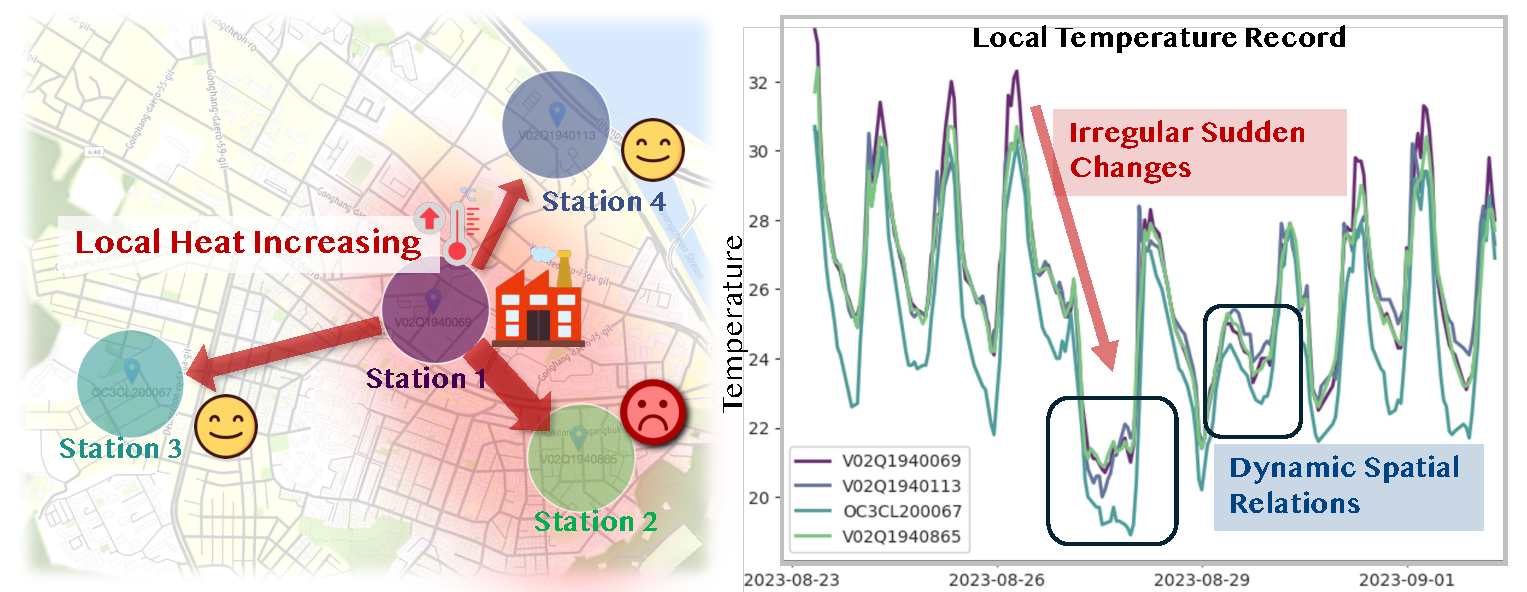
\includegraphics[width=1.0\linewidth]{resources/intro_1.pdf}
    \vspace{-1em}
    \caption{Introduction of Urban Heat Island effect. \textit{Left:}  Regional UHI effects are closely linked to the regional environment. \textit{Right:} Urban thermodynamics is temporal irregular and has highly dynamic spatial relations.}
    \label{fig:intro_data}
    \vspace{-1.5em}
\end{figure}

Rapid urbanization has caused a host of environmental and sustainability challenges in cities and beyond~\cite{krupat1985people,keivani2009review,zheng2014urban,wen2023diffstg,zou2024learning,zou2025deep}. Within cities, the dynamic interaction between natural elements and human activities leads to localized heat accumulation, thereby giving rise to the sophisticated \textbf{Urban Heat Island (UHI)} effect~\cite{lyu2022integrated,yoo2018investigating,li2019urban}. 
Recognizing the critical importance of this issue, the United Nations has identified "\textit{cities and human settlements climate resilient and sustainable}" as a key sustainable development goal~\cite{lu2015policy}. This mandate, coupled with the challenges posed by global warming ~\cite{alcoforado2008global,santamouris2014energy,santamouris2015impact} and the increasing vulnerability of elderly and at-risk populations~\cite{zhu2023urban,park2021differing,heaviside2017urban}, underscores the urgent need to develop robust thermodynamic models for accurate UHI forecasting.


Forecasting the UHI effect, usually quantified through urban field temperatures, presents distinct challenges compared to conventional climate forecasting. Most existing studies have predominantly utilized macro-scale and qualitative approaches, either by contrasting temperatures between urban cores and their surrounding suburban areas~\cite{rizwan2008review,yang2016research,tehrani2024predicting} or by interpolating land temperatures using remote sensing observations~\cite{mirzaei2010approaches,peng2012surface,diem2024remote,zhou2018satellite}. However, both the UHI effect and the associated field temperature demonstrate remarkable variability within urban areas, exhibiting gradients that reflect differing levels of urban development~\cite{lyu2022integrated,yoo2018investigating}. Neighborhood-specific factors, such as the presence of green spaces, water bodies, and land function, further contribute to this spatial heterogeneity. Consequently, the inherent complexity of these urban thermodynamics renders coarse-grained remote sensing data and traditional numerical inference methods~\cite{adilkhanova2022recent,yang2022quantitative} insufficient for this application.

Recently, data-driven methods such as GenCast~\cite{price2025probabilistic} and Pangu-weather~\cite{bi2022pangu,xu2024improvement} have shown impressive accuracy in climate forecasting by modeling global atmospheric dynamics. However, when addressing regional climate phenomena at low altitudes, they tend to underperform compared to traditional numerical models~\cite{olivetti2024data,huang2025initial}. This discrepancy reveals the significant challenge of modeling urban thermodynamics for fine-grained UHI effect forecasting. As shown in Figure \ref{fig:intro_data}, firstly, UHI patterns are closely intertwined with various environmental factors, leading to complex spatial heterogeneity that further complicates modeling effects. Secondly, fine-grained regional temperature variations are more sensitive and irregular than those found in general atmospheric circulation~\cite{price2023gencast,nguyen2023scaling} or in other spatio-temporal phenomena such as regional traffic flow~\cite{liang2023airformer,yin2021deep,li2023dynamic}.  As a result, key challenges remain in effectively capturing spatio-temporal thermodynamics of local thermal systems and integrating essential environmental information without introducing noise.

\begin{figure}[t!]
    \centering
    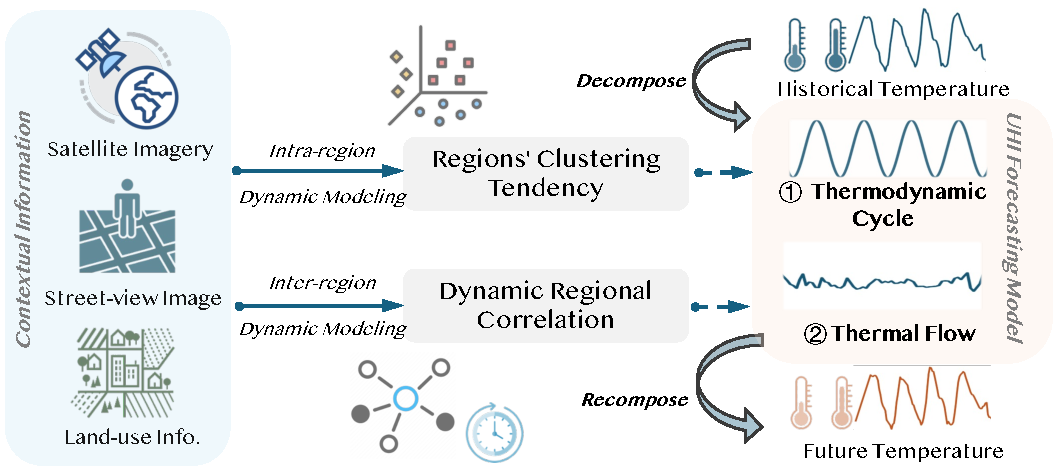
\includegraphics[width=1\linewidth]{resources/intro_2.pdf}
    \vspace{-1em}
    \caption{Insight of the framework.}
    \label{fig:intro_method}
    \vspace{-1.5em}
\end{figure}
In theory, the problem can be addressed using the heat equation by treating spatio-temporal thermodynamics as a flow physics problem. Accurate modeling of local thermodynamics becomes promising by incorporating urban environmental information as boundary conditions for the nonlinear partial differential heat equation~\cite{widder1976heat,doob1955probability,lewis2004fundamentals}, although an analytical solution for such an equation is not achievable. In this paper, guided by this equation, we introduce \model, a data-driven framework for modeling local thermodynamics with contextual information. To enable data-driven instantiation of the partial differential equation, local thermodynamics are decomposed into intra-region \textbf{thermodynamic cycles}~\cite{chen2010review,qian2015thermodynamics} and inter-region \textbf{thermal flows}~\cite{lewis2004fundamentals,zienkiewicz1981general} (see Fig. \ref{fig:intro_method}).

\begin{figure*}
    \centering
    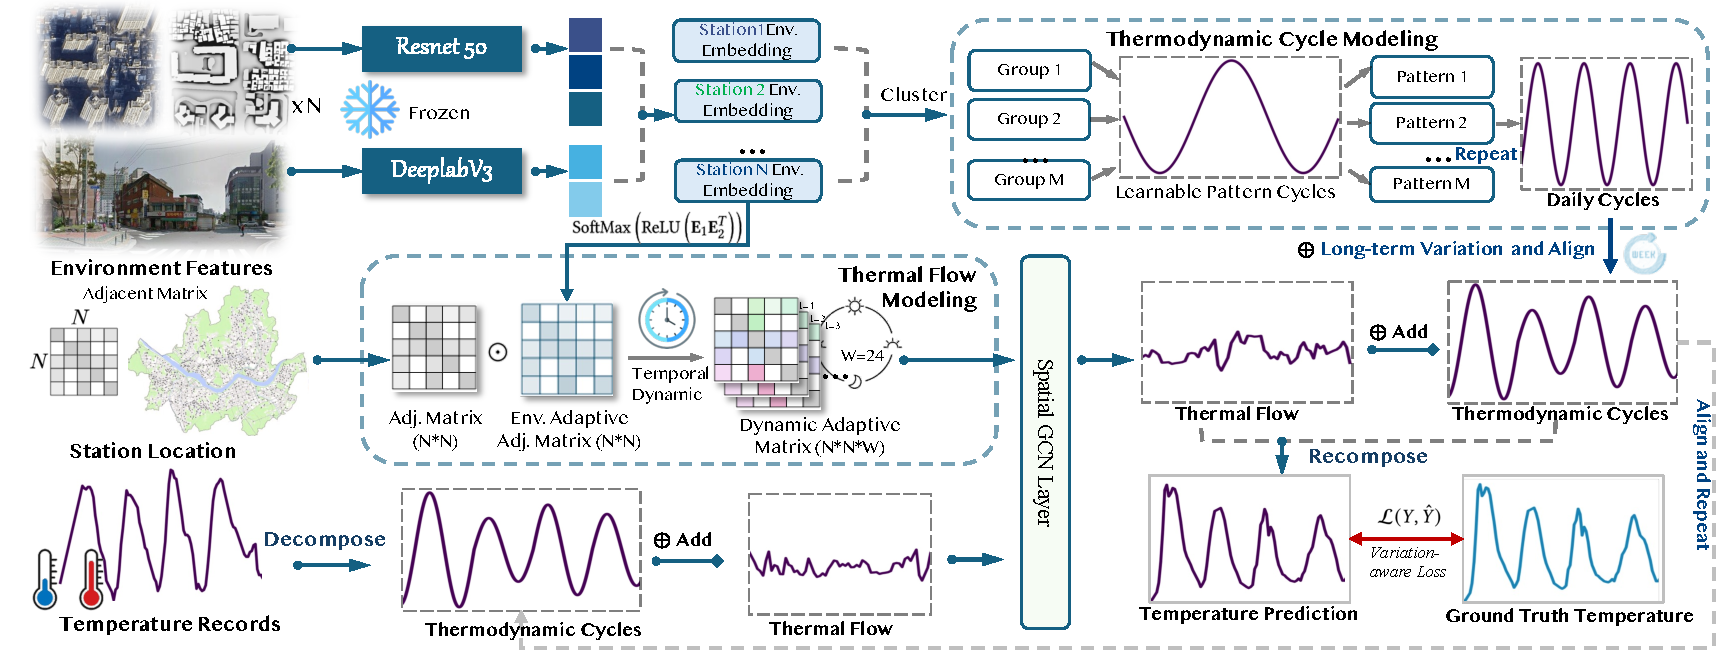
\includegraphics[width=0.95\linewidth]{resources/framework.pdf}
    \vspace{-0.5em}
    \caption{An illustration of our proposed \model framework.}
    \vspace{-1em}
    \label{fig:frame}
\end{figure*}
Firstly, according to thermal equation, without disturbance, the daily thermal cycle of a region is stable and distinct, referred to as the intra-region \textbf{thermodynamic cycle}. This cycle contributes to the daily temperature variations and is determined by the region's Specific Heat Capacity (SHC), which is influenced by the components of the surrounding environment. Inspired by these characteristics, we cluster stations into groups based on their similar environmental features and design a temporal periodicity learning block to explicitly instantiate the different temporal cycles. This approach efficiently models the regional thermodynamic cycle while avoiding complex over-fitting.

Secondly, inter-region \textbf{thermal flow} refers to the thermal transfer process of local heat variation between adjacent regions caused by temperature differences, contributing to irregular temporal variations in temperature. Although these mechanics can be naturally represented through spatial graph convolution~\cite{zou2024learning,song2020spatial,lu2020spatiotemporal,alet2019graph,sanchez2020learning}, heat transfer in regional thermal equation is anisotropic in different directions and times due to various environment situations. This behavior goes beyond the capacity of a vanilla distance-based adjacency matrix. Therefore, we introduce a dynamic adaptive convolution block to instantiate the anisotropic thermal flow. Specifically, we introduce a context-aware adaptive graph convolution to learn the spatial anisotropy from environment features. For the temporal anisotropy, we design lightweight temporal dynamic learning mechanics to represent the temporal variation of heat transfer without introducing redundant model complexity.

Modeling the two thermal mechanics separately provides clear solutions. However, orderly recomposing them for UHI effect forecasting presents another challenge in terms of an imbalanced value range. The temperature temporal fluctuations caused by local thermal flow are minor compared to the daily thermal cycle, which may lead to these fluctuations being misinterpreted as noise by the cycle learning block, and vice versa. While explicitly modeling the daily cycle in our temporal learning block can help mitigate this issue, the training process remains unstable. To address this challenge, we introduce a fluctuation fine-tuning training strategy and a variation-aware loss function within our framework to effectively support our decomposition strategy.

Furthermore, we conduct an in-depth study to demonstrate the necessity and effectiveness of our framework in the context of fine-grain temperature predictions and warnings for extreme heat events. In addition, we deploy it on our SeoUHI platform to deliver real-world UHI effect forecasting and notifications to the citizens in the Seoul area. Our contributions are summarized as follows:




(1) We propose \textit{DeepUHI}, the first data-driven context-aware framework for modeling local thermodynamics based on the heat equation. In our methodology, we introduce an explainable heat decomposition framework to represent thermodynamics from the perspectives of \textit{thermodynamic cycles} and \textit{thermal flows}, which systematically and concisely incorporates urban environmental data into the forecasting process.

(2) We conduct extensive experiments to demonstrate the necessity and effectiveness of our proposed framework. Comprehensive results indicate that it outperforms existing time-series and spatio-temporal forecasting baselines in UHI effect forecasting and warning tasks while maintaining high computational efficiency.

(3) We collect and introduce \textit{SeoulTemp}, the first fine-grained urban temperature dataset that includes field environment data across multiple modalities. This dataset encompasses a total of 947 temperature stations covering 605 $km^{2}$ of land in Seoul from 2021 to 2024, specifically targeting spatio-temporal UHI effect forecasting at the street level in urban areas.

(4) Our framework and model are deployed on the SeoUHI platform, providing precise short-term (day-ahead) UHI effect and extreme temperature notification services for over 10 million citizens in the Seoul area.




% In this work, we first introduce a real-word dataset, called \textit{SeoulTemp}, the first fine-grained, publicly available, and multi-modal dataset specifically targeting spatio-temporal UHI effect predictions for the Seoul area at the street level. As shown in Figure 1,
% the \textit{SeoulTemp} dataset is composed of three modalities of data, i.e.,
% Satellite Imagery, Street-view Imagery, Seoul Land-use Dataset, SDot Temperature Database, covering a total of 947 temperature stations within 605 $km^{2}$ land of Seoul from 2021 to 2024. The satellite and street-view imagery comprehensively describe the environment around each station. The Seoul Land-use Dataset, obtained from the Korea EGIS, offers fine-grain land-use information for each station. The SDot Temperature Dataset, sourced
% from the Seoul SDot project, contains hourly field average temperature of stations.


\section{Preliminaries}
\label{sec:model}

\begin{myDef}
\textbf{Urban Heat Island Effect.} Urban heat island effect refers to the quantification of the local thermal behavior of city within a complex felid environment. A higher level of UHI effect indicates that people or urban infrastructures are likely to experience greater heat effects at that time. In practice, the UHI effect is quantified using field temperature series $\mathbf{X} \in \mathbb{R}^{N \times T}$, where $\mathbf{X}_{i,j}$ denotes the $i_{th}$ attribute at time $j$.
\end{myDef}


\begin{myDef}
\textbf{Thermal Station Network.} Thermal station network consists of a group of local temperature monitoring stations within a city, denoted as $\mathcal{G}=(\mathbf{V},\mathbf{E})$, where $\mathbf{V}$ represents the set of stations and $N =|\mathbf{V}|$ is the number of stations. The set $E$ denotes the edges that represent the relationships among the stations. Here, we use $\mathbf{A} \in \mathbb{R}^{N \times N}$ to denote the basic distance-based adjacency matrix of the thermal station network.
\end{myDef}

\begin{myDef}
\textbf{Contextual Feature.} Contextual features represent the environmental features surrounding each station. In practice, we use satellite imagery, street-view imagery, and land-use information to represent the surrounding environment. These diverse types of features can be flattened and concatenated to form a comprehensive representation. We denote the contextual features associated with each station as $\mathbf{C} \in \mathbb{R}^{N \times C}$, where $C$ represents the feature dimension.
\end{myDef}

\begin{problem}

\textbf{Urban Heat Island Effect Forecasting.} For graph $\mathcal{G}$, we compute pairwise distances between stations to derive the adjacency matrix based on a predefined distance threshold. Let  $\mathbf{X} \in \mathbb{R}^{N \times T}$ denote the observed field temperatures from all stations, where $T$ is the number of historical time steps. The historical observation at time $t$ is defined as $\mathcal{H}^{t} = (\mathcal{G}, \mathbf{C}, \mathbf{X}^{t})$. The forecasting problem is framed probabilistically as:
\begin{equation}
p\left(\mathcal{Y}^{t+1:t+K} \mid \mathcal{H}^{t-P+1:t}\right) = \mathcal{F}_\theta\left(\mathcal{H}^{t-P+1}, \dots, \mathcal{H}^t\right)
\end{equation}
where $p\left(\mathcal{Y}^{t+1:t+K} \mid \mathcal{H}^{t-P+1:t}\right)$ is the predictive probability distribution over future observations. To learn model parameters $\theta$, we maximize the log-likelihood of the observed future sequences:
\begin{equation}
\theta^* = \arg\max_\theta \sum_{t=P}^{T - K} \log p\left(\mathcal{Y}^{t+1:t+K} \mid \mathcal{H}^{t-P+1:t}\right)    
\end{equation}
\end{problem}

% For $\mathcal{G}$, we compute the pairwise distances between stations and derive the adjacency matrix using a predefined distance threshold. Let $\mathbf{X} \in \mathbb{R}^{N \times T}$ be the observed field temperature from all stations, where $T$ represents the number of historical time steps. We denote $\mathcal{H}^{t} = (\mathcal{G}, \mathbf{C}, \mathbf{X}^{t})$, which indicates all the observed values at time step $t$. We define the problem as follows:
% \begin{equation}
% \left(\hat{\mathcal{Y}}^{t+1}, \hat{\mathcal{Y}}^{t+2}, \cdots, \hat{\mathcal{Y}}^{t+K}\right) \leftarrow \mathcal{F}_\theta\left(\mathcal{H}^{t-P+1}, \mathcal{H}^{t-P+2}, \cdots \mathcal{H}^t\right)
% \end{equation}

% where $\hat{\mathcal{Y}}^{t+K}$ denotes the predicted value at time step $t+K$, $\mathcal{F}_\theta$ is the forecasting model, $P$ and $K$ are the number of historical and future time steps, respectively.


% \textbf{Urban Heat Island Effect} refers to the quantification of the local thermal behavior of a city within a complex regional environment. A higher level of UHI effect indicates that people or urban infrastructures are likely to experience greater heat effects at that time. In practice, the UHI effect is quantified using field temperature series.

% \noindent\textbf{Thermal Station Network} consists of a group of local temperature monitoring stations within a city, denoted as $\mathcal{G}=(\mathbf{V},\mathbf{E})$, where $\mathbf{V}$ represents the set of stations and $N =|\mathbf{V}|$ is the number of stations. The set $E$ denotes the edges that represent the relationships among the stations. In this context, we use $\mathbf{A} \in \mathbb{R}^{N \times N}$ to denote the distance-based adjacency matrix of the station network.

% \noindent\textbf{Contextual Feature} represents the environmental features surrounding each station. In practice, we use satellite imagery, street-view imagery, and land use information to represent the surrounding environment. We denote the contextual features associated with each station as $\mathbf{C} \in \mathbb{R}^{N \times C}$, where $C$ represents the feature dimension.

% \textbf{Problem Statement.} For $\mathcal{G}$, we compute the pairwise distances between stations and derive the adjacency matrix using a predefined distance threshold. Let $\mathbf{X} \in \mathbb{R}^{N \times T}$ be the observed field temperature from all stations, where $T$ represents the number of historical time steps. We denote $\mathcal{H}^{t} = (\mathcal{G}, \mathbf{C}, \mathbf{X}^{t})$, which indicates all the observed values at time step $t$. We define the problem as follows.

% \begin{equation}
% \left(\hat{\mathcal{Y}}^{t+1}, \hat{\mathcal{Y}}^{t+2}, \cdots, \hat{\mathcal{Y}}^{t+K}\right) \leftarrow \mathcal{F}_\theta\left(\mathcal{H}^{t-P+1}, \mathcal{H}^{t-P+2}, \cdots \mathcal{H}^t\right),
% \end{equation}

% where $\hat{\mathcal{Y}}^{t+K}$ denotes the predicted value at time step $t+K$ , $\mathcal{F}_\theta$ is the forecasting model, $P$ and $K$ are the number of historical and future time steps, respectively.
\section{Methodology}
\label{sec:solution}



\subsection{Overall Framework}
\paratitle{Theoretical Statement.} The study of the Urban Heat Island (UHI) effect involves understanding thermodynamics as a flow physics problem. In the context of flow physics, where diffusion occurs through a medium, it is common to establish a Cartesian coordinate system to analyze the classical heat function $u(x,y,z,t)$ with three spatial variables $(x,y,z)$ and one time variable $t$. In this setting, $u$ is considered a solution to the heat equation under isotropic conditions if it satisfies the following equation:
\begin{equation}
\frac{\partial u}{\partial t}=\alpha\left(\frac{\partial^2 u}{\partial x^2}+\frac{\partial^2 u}{\partial y^2}+\frac{\partial^2 u}{\partial z^2}\right)
\end{equation}
Here, $\alpha$ is a positive coefficient known as the \textit{thermal diffusivity} of the medium. However, in the context of fine-grain heat dynamics within a city, the assumption of isotropic conditions for air is inaccurate. The heat flow across different regions with varying environments is anisotropic, meaning that $\alpha$ is not a constant coefficient but rather a function that depends on the spatial coordinates $(x,y,z)$. Consequently, the equation assumes a nonlinear partial differential form that does not possess a precise analytical solution~\cite{reitzle2019semi}:
\begin{equation}
\label{heat_equ}
\frac{\partial u}{\partial t}=\frac{\partial}{\partial x}\left(\alpha(x, y, z) \frac{\partial u}{\partial x}\right)+\frac{\partial}{\partial y}\left(\alpha(x, y, z) \frac{\partial u}{\partial y}\right)+\frac{\partial}{\partial z}\left(\alpha(x, y, z) \frac{\partial u}{\partial z}\right)
\end{equation}
where $\alpha(x, y, z)$ represents the value's variation of \textit{thermal diffusivity} at different spatial locations.

Our thermodynamic modeling approach is founded on this equation. First, for a specified region, under steady-state conditions where we exclude influences from other regions, the temperature field will remain constant over time, which implies that $\frac{\partial u}{\partial t}=0$. In this context, the temperature in that region will converge to a stable daily cycle, referred to as the intra-region \textbf{\textit{thermodynamic cycle}}. 
Second, by removing the inner thermodynamic cycle for each station, the remaining variations are attributed to spatial heat flow, as described by Equation \ref{heat_equ} where $\frac{\partial u}{\partial t}\neq 0$. This heat flow characterizes the transfer of heat between urban regions, such as industrial heat flow from urban areas to suburban areas during peak times. We refer to this anisotropic flow as inter-region \textbf{\textit{thermal flow}}.


\paratitle{Framework Design.} The overall architecture of our proposed model is depicted in Figure \ref{fig:frame}. Initially, we extract contextual features from multi-modal data to create station environment embeddings to support the modeling of Equation \ref{heat_equ}. Based on the theoretical statement, we decompose the temperature records into \textit{thermodynamic cycles} and \textit{thermal flows}. To model these components in our framework, we introduce a temporal periodicity modeling block for the \textit{\textbf{thermodynamic cycles}} ($\frac{\partial u}{\partial t}=0$) and a dynamic adaptive convolution block for the \textit{\textbf{thermal flows}} ($\frac{\partial u}{\partial t}\neq 0$). Additionally, we incorporate a spatial fine-tuning strategy with a variation-aware loss to facilitate the training of our framework.


\subsection{Contextual Feature Representation}
Contextual features are utilized to reveal the similarities or differences between regions for this research. The primary focus is to identify separability in geospatial space rather than intricate regional details. Therefore, we design a straightforward pipeline to extract contextual feature embeddings $\mathbf{C} \in \mathbb{R}^{N \times C}$ with minimal computational cost.

We employ ResNet50 and DeepLabV3 to unsupervisedly extract visual features from satellite and street-view imagery, respectively. For land use semantic information, inspired by \cite{zou2024learning}, we apply one-hot encoding to differentiate land types and multiply them by their area proportions. We normalize the extracted embeddings from different data sources to align their scales before concatenating them into $\mathbf{C_{\textit{origin}}}$. Subsequently, we use t-SNE to reduce the dimension of $\mathbf{C_{\textit{origin}}}\rightarrow\mathbf{C}\in \mathbb{R}^{N \times C}$, with the aim of enhancing separability, where $C$ is the compressed dimension of the contextual feature.

\subsection{Thermodynamic Cycle Modeling}
\subsubsection{Context-aware Region Grouping}
Conventional multi-channel models typically model each channel individually. This approach can introduce greater complexity and noise as the number of channels increases. This issue is particularly significant when modeling the thermodynamic cycle of temperature across various regions within a city, as numerous environmental studies have shown that temperature cycles in most regions of a city are synchronous \cite{gomez2004experimental,yang2023urban,dimoudi2013investigation}. Therefore, similar regions should share the same thermodynamic cycle modeling; otherwise, respective modeling may capture more noise from the transient inter-region thermal flow. In practice, this similarity is determined by their contextual environment features \cite{gomez2004experimental,heisler2010urban}.

To learn the thermodynamic cycle within a city, we first conduct context-aware region grouping to divide stations and their corresponding regions into $\textbf{M}$ groups based on the context embedding $\mathbf{C}$ using K-Means clustering. The subsequent cycle modeling is then performed for each group rather than for each region. This reduces the computational complexity from $\mathcal{S} \times N$ to $\mathcal{S} \times \textbf{M}$, where $\mathcal{S}$ represents the complexity associated with modeling a single channel. More importantly, by explicitly setting the cycle modeling of similar regions to be the same, the framework becomes more robust to local fluctuations caused by noise or inter-region thermal flow.
\subsubsection{Temporal Periodicity Modeling.}\label{sec:temporal_cycle} Our goal is to identify the underlying stable thermal periodicity for each regional group. Although recent works such as Autoformer and PatchTST have emphasized the importance of data periodicity for long-term time series forecasting, their reliance on heavy Transformer backbones is computationally expensive and sensitive to noise. Additionally, these models lack interpretability, which is crucial for real-world deployment. Inspired by \cite{lincyclenet}, we directly employ learnable daily cycles to explicitly model the temporal periodic pattern of the thermodynamic cycle.

\paratitle{Daily Patterns Modeling.} Given $\textbf{M}$ groups with a daily cycle length $W=24$, we first generate learnable daily cycles $\mathbf{Q} \in \mathbb{R}^{M \times D}$, all initialized to zeros. This can be mapped to $\mathbf{Q} \in \mathbb{R}^{N \times D}$ according to the group mapping $M \Rightarrow N$. These daily cycles are globally shared among groups, which allows us to perform cyclic replications to obtain cyclic components $\textbf{C}$ of the sequence $\textit{X}$ of the same length. The recurrent cycles $\mathbf{Q}$ undergo gradient backpropagation training alongside the backbone module for prediction, yielding learned explicit representations that reveal the internal cyclic patterns within the sequence.

When deriving subsequences $\textbf{C}$ from the cyclic replications of sequence $\mathbf{Q}$, we cannot directly ensure that they maintain the same periodic phase. To address this, we need to align $\mathbf{Q}$ by determining an alignment offset $t\mod W$, where $t$ is the current time point. After alignment, we extract the required subsequences from the aligned sequence ${Q}^{(t)}$. Mathematically, this process can be represented as:
\begin{equation}
\setlength\abovedisplayskip{0pt}
Q^{(t)} = \operatorname{Roll}(Q, t \bmod W),
C_{t-L+1: t} = [\overbrace{Q^{(t)} \cdots Q^{(t)}}^{\lfloor L / W \rfloor \text{ times}}, Q_{0: L \bmod W}^{(t)}]
\end{equation}

\paratitle{Long-term Variation Modeling.} In addition to daily patterns, regional temperature exhibits weekly variations due to human activity and significant seasonal changes resulting from climate change. While these variations may not be significant for short-term predictions over several days, they become important when learning a stable daily cycle from data collected over several years. Otherwise, the regression of the daily cycle \( \mathbf{Q} \) may become unstable as data transitions from summer to winter.

Seasonal variation manifests as a shift in the overall data distribution. To address this, we utilize Reversible Instance Normalization (RevIN)~\cite{kim2021reversible} for each input data sequence to mitigate the effects of seasonal variation, defined by the following equation:
\begin{equation}
x = (x - \frac{1}{T} \sum_{t=1}^{T} x_t)/{\sqrt{\frac{1}{T} \sum_{t=1}^{T} (x_t - \frac{1}{T} \sum_{t=1}^{T} x_t)^2 + \psi }}
\end{equation}

Here, \( \psi \) is the normalization constant that ensures stabilization.
To address the issue of weekly variation, we introduce a weekly variation filtration layer that models and filters out weekly fluctuations, thereby facilitating a more accurate learning of the daily pattern. We compute the time embedding for the day of the week using \( E_{\text{day}} = \operatorname{Emb}(t_{\text{day}} \bmod 7, pos) \) and learn the weights and biases for the weekly daily cycle using the following equations:
\begin{equation}
\mathcal{W}_{\text{cycle}} = \text{ReLU}\left(\mathrm{Linear}_w(E_{\text{day}})\right), \quad \mathcal{B}_{\text{cycle}} = \text{ReLU}\left(\mathrm{Linear}_b(E_{\text{day}})\right)
\end{equation}

Next, for each daily cycle, we update the cycle values in sequence $\textbf{Q}^{t}$ to account for the weekly variation using the equation:
\begin{equation}
\textbf{Q}^{t} = Q^{t} \cdot \mathcal{W}_{\text{cycle}} + \mathcal{B}_{\text{cycle}}.
\end{equation}

\subsection{Thermal Flow Modeling}

\subsubsection{Residual Fluctuation Learning.}
Thermal flow refers to the process of heat transfer that occurs due to temperature differences between adjacent regions. This process is similar to local fluctuations in the stable climate system. Unlike the thermodynamic cycles observed within a single region, the global value variation resulting from thermal flow is typically minor, often limited to single-digit changes. As a result, traditional time series forecasting models for weather or climate prediction frequently overlook the individual modeling of thermal flow.

We introduce residual wave learning to address this issue as shown in Equation \ref{equ:res}. Based on thermodynamic cycle modeling, we remove the cycle components $\textbf{Q}^{t}$ from the observed field temperature $\textbf{X} \in \mathbb{R}^{N \times P}$ to enhance the $\mathcal{F}$ model's attention on the spatio-temporal wave caused by thermal flow. The output results of the backbone will be combined with the inferred cycle component $\textbf{Q}^{t+P}$ to obtain the final prediction $\hat{\textbf{X}} \in \mathbb{R}^{N \times K}$. 
\begin{equation}
\label{equ:res}
    \hat{\textbf{X}} = \mathcal{F}(\textbf{X} - \textbf{Q}^{t}) + \textbf{Q}^{t+P}
\end{equation}

\subsubsection{Periodic Dynamic Graph Learning.}
\label{sec:spatial_cycle}
To model thermal flow, it is necessary to introduce graph learning in $\mathcal{F}$. However, static and distance-based graph learning structures, such as conventional STGCNs, cannot effectively represent the anisotropy of thermal flow mechanics in both spatial and temporal dimensions. This anisotropy arises from the spatio-temporal variation of thermal diffusivity, as described in Equation \ref{heat_equ}. Although advanced works, such as GraphWaveNet~\cite{wu2019graph}, introduce adaptive adjacency matrices to automatically learn the spatial relationships between nodes, they are limited in representing the spatial variance of $\alpha(x, y, z)$ and do not account for the time variation in $u(x,y,z,t)$ of the heat equation. Directly incorporating temporal dynamic graph learning to represent $t$ can lead to a model that is overly complex for multiple time steps and difficult to train. We design a periodic dynamic graph learning framework to address the modeling of thermal flow.

\paratitle{Context-aware Adaptive Graph.} We adapt the basic self-adaptive adjacency matrix learning method from~\cite{wu2019graph} as the base matrix to represent spatial variance $\alpha(x, y, z)$ at static time $t$ and enhance it with context information awareness. The adaptive adjacency matrix is computed as:
\begin{equation}
\tilde{\mathbf{A}}_{a d p}=\operatorname{SoftMax}\left(\operatorname{ReLU}\left(\mathbf{E}_1 \cdot \mathbf{E}_2^T\right)\right) \odot \mathbf{A}
\end{equation}
where $\mathbf{E}_1$ and $\mathbf{E}_2$ are node embeddings obtained through linear transformations of the contextual feature $\mathbf{C} \in \mathbb{R}^{N \times C}$. It is important to note that we multiply the learned matrix by the original distance-based matrix $\mathbf{A}$ to maintain sparsity.

\paratitle{Temporal Periodic Dynamic Learning.} To account for the temporal variation in thermal flow mechanics, we need to introduce variable $t$ to adjust the learned spatial relations in $\tilde{\mathbf{A}}_{a d p}$ at different time step $t$. However, the task becomes overly complex for increasing time steps. Therefore, we design a periodic dynamic learning method to manage complexity while accommodating an increasing number of time steps $t$.

In practice, regional thermal flow continuously varies over time while also exhibiting regularity similar to intra-region thermodynamic cycles. This regularity results from the consistent warming and cooling periods that occur daily, leading to periodic thermal flow variation. Consequently, we expand $\tilde{\mathbf{A}}_{a d p}\rightarrow\tilde{\mathbf{A}}^{I}_{a d p} \in \mathbb{R}^{N \times N \times W}$, where $W$ is consistently set to 24, akin to thermodynamic cycle modeling, to represent the regular daily dynamics of thermal flow. For each $i \in W$, which represents the time of day, we individually construct $\tilde{\mathbf{A}}_{a d p}^{i}$ for this time period and perform spatial convolution based on it when each time step $t$ satisfies $t \bmod W = i$. Thus, the number of $\tilde{\mathbf{A}}_{a d p}^{i}$ is limited to 24, offering a clear and efficient solution for the temporal dynamic representation.

Additionally, to extract fluctuation properties while maintaining efficiency, we employ a simple 2-layer MLP as the temporal backbone for the residual thermal flow series ${\textbf{X} - \textbf{Q}^{t}}$, denoted as $\textbf{X}_{res}$ below. The overall model's temporal periodic dynamic learning process can be formulated as:
\begin{equation}
\hat{\textbf{X}}_{res}^{t} = \operatorname{Conv}(\textbf{X}^{t}_{res}, \tilde{\mathbf{A}}_{a d p}^{t \bmod W}),\quad \hat{\textbf{Y}}_{res} = \operatorname{MLP}(\hat{\textbf{X}}_{res})
\end{equation}

\subsection{Fine-tuning and Variation-aware Loss}
\subsubsection{Fluctuation Fine-tuning}
Our residual learning framework enables the separate learning of thermodynamic cycles and thermal flow, which are decomposed and recomposed to predict the urban heat island (UHI) effect. However, the imbalance between these components can impede training. Local thermal flow fluctuations are minor compared to the daily thermal cycle, leading to potential misinterpretation as noise by the cycle learning block, and vice versa.

Additionally, the temporal cycle learning block may overly adapt to temporal variations, hindering the thermal flow learning block's ability to model spatial relationships. This issue is partly addressed through our explicit daily pattern modeling strategy, which restricts the daily cycle modeling capacity of $\mathbf{Q}$. To enhance performance,     it is crucial to address this during training.
Therefore, we introduce fluctuation fine-tuning. We freeze the gradient updates of the temporal cycle learning block for 20 epochs during the fine-tuning stage to reduce the impact of temporal overfitting on thermal flow modeling. The residual framework remains unchanged, allowing the model to focus on capturing meaningful relationships within the static residual components.

\subsubsection{Variation-aware Loss.} Time series (TS) or spatial-temporal (ST) models typically minimize \(L_p\) norm distances as loss functions, such as Mean Absolute Error (MAE) or Mean Squared Error (MSE) for training. However, point-wise comparisons are insufficient for identifying continuous variations, such as trends and cycles, which can lead to uninformative predictions that do not account for temporal dynamics like peaks and troughs. For urban heat island (UHI) effect forecasting, we focus more on variation dynamics rather than single-value precision. Therefore, we need to design a variation-aware loss that considers both point-wise distances and temporal variations.

Inspired by \cite{lee2022tilde}, we construct our loss using Amplitude Shifting Invariance \(\mathcal{L}_{amp}\), Phase Shifting Invariance \(\mathcal{L}_{phase}\), and Point-wise Distance \(\mathcal{L}_{point}\). Our variation-aware loss is formulated as follows:
\begin{equation}
    \mathcal{L}(Y, \hat{Y}) = \alpha \mathcal{L}_{amp}(Y, \hat{Y}) + (1 - \alpha) \mathcal{L}_{phase}(Y, \hat{Y}) + \gamma \mathcal{L}_{point}(Y, \hat{Y})
\end{equation}
\begin{equation}
    \mathcal{L}(Y, \hat{Y}) = \alpha \mathcal{L}_{amp} +  \mathcal{L}_{phase} + \mathcal{L}_{point}
\end{equation}
where \(\alpha,\gamma \in [0,1]\) are hyperparameters. We provide the introduction and equations for each loss component in Appendix \ref{app:loss}.
\section{Experiments}

% Please add the following required packages to your document preamble:
% \usepackage{multirow}
% \usepackage{graphicx}
% \usepackage[normalem]{ulem}
% \useunder{\uline}{\ul}{}
\begin{table*}[]
\centering

\small
\caption{Regional Temperature
Prediction. The best results are in \textbf{bold} and second-best results are {\ul underlined}.}
%\vspace{-1em}
\label{exp_mae}
\resizebox{0.95\textwidth}{!}{%
\begin{tabular}{cccccccccccc}
\hline
\multirow{2}{*}{Horizons} & \multirow{2}{*}{Metric} & \multicolumn{3}{c}{\textit{Traditional Methods}} & \multicolumn{2}{c}{\textit{Time-series Methods}} & \multicolumn{4}{c}{\textit{Spatio-temporal Methods}} & \multirow{2}{*}{DeepUHI} \\ \cline{3-11}
 &  & HA & LR & ARIMA & DLinear & PatchTST & GWN & MTGNN & STID & STAEformer &  \\ \hline
\multirow{2}{*}{12} & MAE & 3.535 & 1.599 & 3.453 & 1.653 & 1.774 & 1.642 & 1.639 & \textbf{1.431} & 1.456 & {\ul 1.433} \\
 & sMAPE & 0.485 & 0.408 & 0.486 & 0.256 & 0.309 & 0.257 & 0.261 & {\ul 0.242} & 0.244 & \textbf{0.241} \\ \hline
\multirow{2}{*}{24} & MAE & 3.672 & 2.031 & 3.563 & 2.015 & 2.111 & 2.014 & 1.987 & {\ul 1.875} & 1.944 & \textbf{1.811} \\
 & sMAPE & 0.497 & 0.332 & 0.499 & 0.321 & 0.344 & 0.322 & 0.309 & {\ul 0.305} & 0.312 & \textbf{0.303} \\ \hline
\multirow{2}{*}{48} & MAE & 3.884 & 2.693 & 3.991 & 2.735 & 2.748 & 2.601 & 2.552 & {\ul 2.495} & 2.499 & \textbf{2.367} \\
 & sMAPE & 0.514 & 0.403 & 0.524 & 0.412 & 0.434 & 0.405 & 0.392 & 0.387 & {\ul 0.382} & \textbf{0.375} \\ \hline
\multirow{2}{*}{96} & MAE & 4.210 & 3.431 & 4.325 & 3.428 & 3.670 & 3.419 & 3.335 & 3.331 & {\ul 3.264} & \textbf{3.231} \\
 & sMAPE & 0.543 & 0.484 & 0.555 & {\ul 0.477} & 0.513 & 0.493 & {\ul 0.477} & 0.483 & 0.478 & \textbf{0.464} \\ \hline
\end{tabular}%
}
\end{table*}
\label{sec:eval}
In this section, we evaluate our proposed \model to address the following research questions:
\begin{itemize}[leftmargin=*]
    \item \textbf{RQ1}: Can \model outperform the latest time-series (TS) or spatio-temporal (ST) forecasting models on the regional temperature prediction task using real-world datasets?
    \item \textbf{RQ2}: How does the performance of \model in UHI warning tasks, from both spatial and temporal dimensions, compare to state-of-the-art TS or ST forecasting models?
    \item \textbf{RQ3}: Can \model clearly learn the thermodynamic cycle and spatial thermal flow relations using the heat decomposing framework to model the fine-grained thermal dynamics?
    \item \textbf{RQ4}: How effective are the designs of \model under various ablation settings?
    
\end{itemize}

\subsection{Experimental Settings}
\subsubsection{Dataset}
\textit{SeoulTemp} dataset consists of three data modalities, covering 947 temperature stations across 605 $km^2$ of Seoul from 2021 to 2024. The satellite and street-view imagery provide detailed environmental context for each station. The Seoul Land-use Dataset, obtained from Korea EGIS, offers fine-grained land-use information for each station. The SDot Temperature Dataset, sourced from the Seoul SDot project, includes hourly average temperatures for the stations. With an average distance of approximately 500 meters between deployed stations, satellite imagery, street-view data, and land-use information are assigned to each station at a 500 m $\times$ 500 m grid scale. The temperature dataset spans from January 1, 2021, to April 8, 2024, with values ranging from $-19.9 \sim +43.2$ \textcelsius. The maximum temperature difference between stations exceeds $10$ \textcelsius during both winter and summer.
\subsubsection{Implementation Details}
Experiments are conducted on the SeoulTemp Dataset. The dataset is divided into training, validation, and test sets with a ratio of $8:1:1$. We fix the look-back length of data to 96 steps to fairly compare the models. \model is implemented using PyTorch, with the Adam optimizer selected for optimization. The learning rate and weight decay are set to 0.01 and 0.0001, respectively. The batch size is fixed at 256, and the embedding dimension of the environmental features is set to 8. For the number of node groups, we follow the taxonomy studies~\cite{li2024deep,pauleit2000assessing} of urban region landscapes to divide the nodes into 10 to 25 groups, and we standardize this to 10 for simplicity.

\subsubsection{Baseline Methods} We include diverse baseline models from various research lines to ensure an extensive comparison. For traditional statistic methods, we include Historical Average (HA), Linear Regression (LR), and Auto-Regressive Integrated Moving Average (ARIMA). For TS methods, we include DLinear~\cite{zeng2023transformers} and PatchTST~\cite{nie2022time} as the representative TS models. For ST methods that are devised for spatio-temporal forecasting tasks, we adopt GWN~\cite{wu2019graph} and MTGNN~\cite{wu2020connecting} as the state-of-the-art STGCNs model. We also include STID~\cite{shao2022spatial} and STAEformer~\cite{liu2023spatio} as state-of-the-art spatio-temporal embedding-based ST methods. We describe the baselines as follows:
\begin{itemize}[leftmargin=*]
\item \textbf{HA}. This method uses the average value of the historical data as the predicted value for future time points.
\item \textbf{LR}. It uses historical data to estimate the coefficients of the linear equation and predicts future values based on this equation.
\item \textbf{ARIMA}. A popular time series forecasting model that combines autoregression, differencing, and moving average components to capture the temporal dependencies and trends in the data.
\item \textbf{DLinear~\cite{zeng2023transformers}}: A method that employs fully connected neural networks with moving average to capture the temporal patterns and dependencies in the data and has shown stable performance in various time series forecasting tasks.
\item \textbf{PatchTST~\cite{nie2022time}}. A widely adapted model that utilizes temporal transformer and patching technique to effectively capture the long-range dependencies and local patterns in time series data. It divides the time series into patches and uses self-attention mechanisms to model the relationships between these patches.
\item \textbf{GWN~\cite{wu2019graph}}. A spatio-temporal graph convolutional network that uses dilated convolutions and adaptive graph convolutional networks to capture the spatial and temporal dependencies in spatio-temporal data. It is designed for spatio-temporal forecasting tasks and has achieved robust performance in many datasets.
\item \textbf{MTGNN~\cite{wu2020connecting}}. A advanced spatio-temporal graph convolutional network with an efficient graph learning layer to automatically extract the relationships between variables. The model uses a mix-hop propagation layer and dilated inception layers to effectively model the complex dependencies in the data.
\item \textbf{STID~\cite{shao2022spatial}}. A spatio-temporal embedding-based model that captures the spatio-temporal dependencies by learning spatio-temporal embeddings and using them as input to a neural network for prediction. It is designed to jointly handle the complex interactions and dependencies in spatio-temporal data.
\item \textbf{STAEformer~\cite{liu2023spatio}}. A spatio-temporal embedding-based model that leverages self-attention mechanisms to capture long-range dependencies, enhancing predictive performance by integrating transformer strengths and achieving SOTA performance.
\end{itemize}

\subsubsection{Evaluation Protocols}
For temperature prediction tasks, we adopt the commonly used Mean Absolute Error (MAE) and symmetric Mean Absolute Percentage Error (sMAPE) to evaluate the models. Lower values in MAE and sMAPE indicate higher prediction accuracy. For UHI warning tasks, we quantify the accuracy in identifying the hottest location and time in both spatial and temporal dimensions using Spatio-temporal Top-K Accuracy (STTop-K):
\begin{equation}
\mathcal{A}= \frac{1}{B} \sum_{b=1}^{B} \mathbb{I}\left( \bigcup_{i=1}^{k} \left( \mathcal{D}[\mathbf{Y}_{b, i}, \hat{\mathbf{Y}}_{b, 0}] \leq \mathcal{D}{\theta} \right) \land \left( \left| \mathcal{T}[\mathbf{Y}_{b, i}, \hat{\mathbf{Y}}_{b, 0}] \right| \leq \mathcal{T}{\theta} \right) \right)
\end{equation}
Here, $\mathbf{Y}_{b, 0}$ represents the hottest point in batch $b$, and $\hat{\mathbf{Y}}_{b, i}$ represents the top $i$ hottest points in the prediction result. The terms $\mathcal{D}$ and $\mathcal{T}$ denote their spatial and temporal distances, while $\mathcal{D}{\theta}$ and $\mathcal{T}{\theta}$ are the corresponding thresholds. The function $\mathbb{I}$ is the indicator function. We use STTop-K to evaluate the matching condition between the top K predicted values and the maximum true value. This method provides a more accurate reflection of the model's UHI warning quality and enhances robustness.

\subsection{Results on Temperature Prediction (RQ1)} We first examine the performance of \model on the regional temperature value prediction task, which is comparable to conventional end-to-end TS or ST forecasting tasks. For a fair comparison, we adhere to the same deployment of baseline models as used in BasicTS~\cite{shao2024exploring}.
% Since temporal convolution based ST models like Graph WaveNet are proven to be over-sophisticate with high look-back length, we utilize a lighter convolution setting to improving their training performance and keep their adaptive spatial convolution advantages following~\cite{XXXX}. Specifically, we train the models XXXX. 
The results summarized in Table~\ref{exp_mae} confirm that our model outperforms both the TS and ST baselines. Specifically, when compared to the previous state-of-the-art STID, the variants of our model demonstrate improvements of over 5\% across most metrics. This indicates the effectiveness of our model in integrating environmental features and heat equation theory into the framework. We attribute the improved performance to the robust thermal decomposing framework, which offers a clearer optimization path for modeling thermal dynamics. Additionally, the variation-aware loss enables our model to effectively capture thermal variation information within the temperature time series, ultimately enhancing model training and downstream performance.

% Please add the following required packages to your document preamble:
% \usepackage{multirow}
% \usepackage{graphicx}
% \usepackage[normalem]{ulem}
% \useunder{\uline}{\ul}{}
\begin{table}[!b]
\vspace{-1em}
\small
\centering
\caption{UHI Warning Spatio-temporal Precision Evaluation.}
\vspace{-1em}
\label{tab:location}
\resizebox{\columnwidth}{!}{%
\begin{tabular}{cccccc}
\hline
\multirow{2}{*}{Method} & \multirow{2}{*}{\begin{tabular}[c]{@{}c@{}}Complexity\\ (multi-adds)\end{tabular}} & \multicolumn{2}{c}{24 Hours} & \multicolumn{2}{c}{48 Hours} \\ \cline{3-6} 
 &  & k=3 & k=9 & k=3 & k=9 \\ \hline
LR & 1.69 M & 0.395 & 0.513 & 0.294 & 0.331 \\
DLinear & 1.69 M & 0.414 & 0.532 & 0.322 & 0.359 \\
GWN & 297,160 M & 0.459 & 0.593 & 0.355 & 0.386 \\
STID & 7,560 M & 0.421 & 0.556 & 0.331 & 0.358 \\
SATEformer & 236,330 M & 0.472 & 0.604 & 0.376 & 0.423 \\ \hline
\multicolumn{6}{c}{Contextual Features Augmented Variants} \\ \hline
DLinear+Context & 13.01M & 0.423 & 0.545 & 0.329 & 0.365 \\
SATEformer+Context & 236,352M & {\ul 0.481} & {\ul 0.644} & {\ul 0.389} & {\ul 0.452} \\ \hline
\textbf{DeepUHI} & 20.95 M & \textbf{0.653} & \textbf{0.802} & \textbf{0.495} & \textbf{0.569} \\ \hline
\end{tabular}%
}
\end{table}
\subsection{Results on UHI Warning (RQ2)}
We further investigate the topic in RQ2, which examines whether our model can achieve more stable performance on future UHI warnings compared to other statistical models from both spatial and temporal perspectives. Unlike urban traffic prediction tasks, the UHI effect and regional temperature prediction encounter more unpredictable variations due to meteorological climate change. Therefore, focusing solely on the accuracy of temperature values is insufficient and unreliable for real-world deployment. Users are more interested in the future trends of the UHI effect, specifically regarding when and where conditions may become excessively hot and hazardous. To address this, we introduce the Spatio-temporal Top-K Accuracy (STTop-K) metrics to quantify the model's performance in identifying the hottest points in both spatial and temporal dimensions. The results are presented in Table~\ref{tab:location}. 
Since existing conventional task-oriented models are usually incompatible to use environment context information of these tasks that may be highly related to the environment, we include context feature augmented with strong TS and ST models for fair and comprehensive evaluation. From the results, we can summarize two significant merits of \model:


\begin{itemize}[leftmargin=*]
    \item \textbf{Superior spatial temporal warning accuracy compared to existing models.} We can observe that the proposed \model can obtain superior results when comparing with state-of-the-art transformer-based ST models that are larger in size and trained for a longer time. Specifically, \model outperforms STAEfomer by a significant margin, which is \underline{35.7\%} over 24-hour-prediction accuracy (k=3). This proves our thermal decomposing strategy and training framework effectively boost the model's understanding of regional thermal dynamics. Our model can quickly size the key variant component of regional temperature and provide more stable forecasting. 
    \item \textbf{Light-weight but most efficient.} It is also noticeable that \model with only 20.95 million of multi-adds for computation achieves even stronger performances than baseline models with huge complexity. \model is reported to be significantly stronger on accuracy with TS models with huge computation cost like GWN. Although RLinear is light in size as \model and widely reported to achieve good performance in conventional time-series forecasting tasks, it shows unsatisfactory performance on this task. It is noticeable that our model also outperforms the contextual feature augmented variants. This proves the advantage of our context-aware framework to efficiently integrate environment information for this task.
\end{itemize}

\subsection{Interpretability of Decomposing (RQ3)}
To prove our theoretical decomposing assumption based on the heat equation and clarify the effectiveness of thermal decomposing mechanisms in enhancing model performance, we provide a comprehensive study of the thermal cycle modeling block and the dynamic heat flow learning block in this section.

\begin{figure}[h]
    \centering
    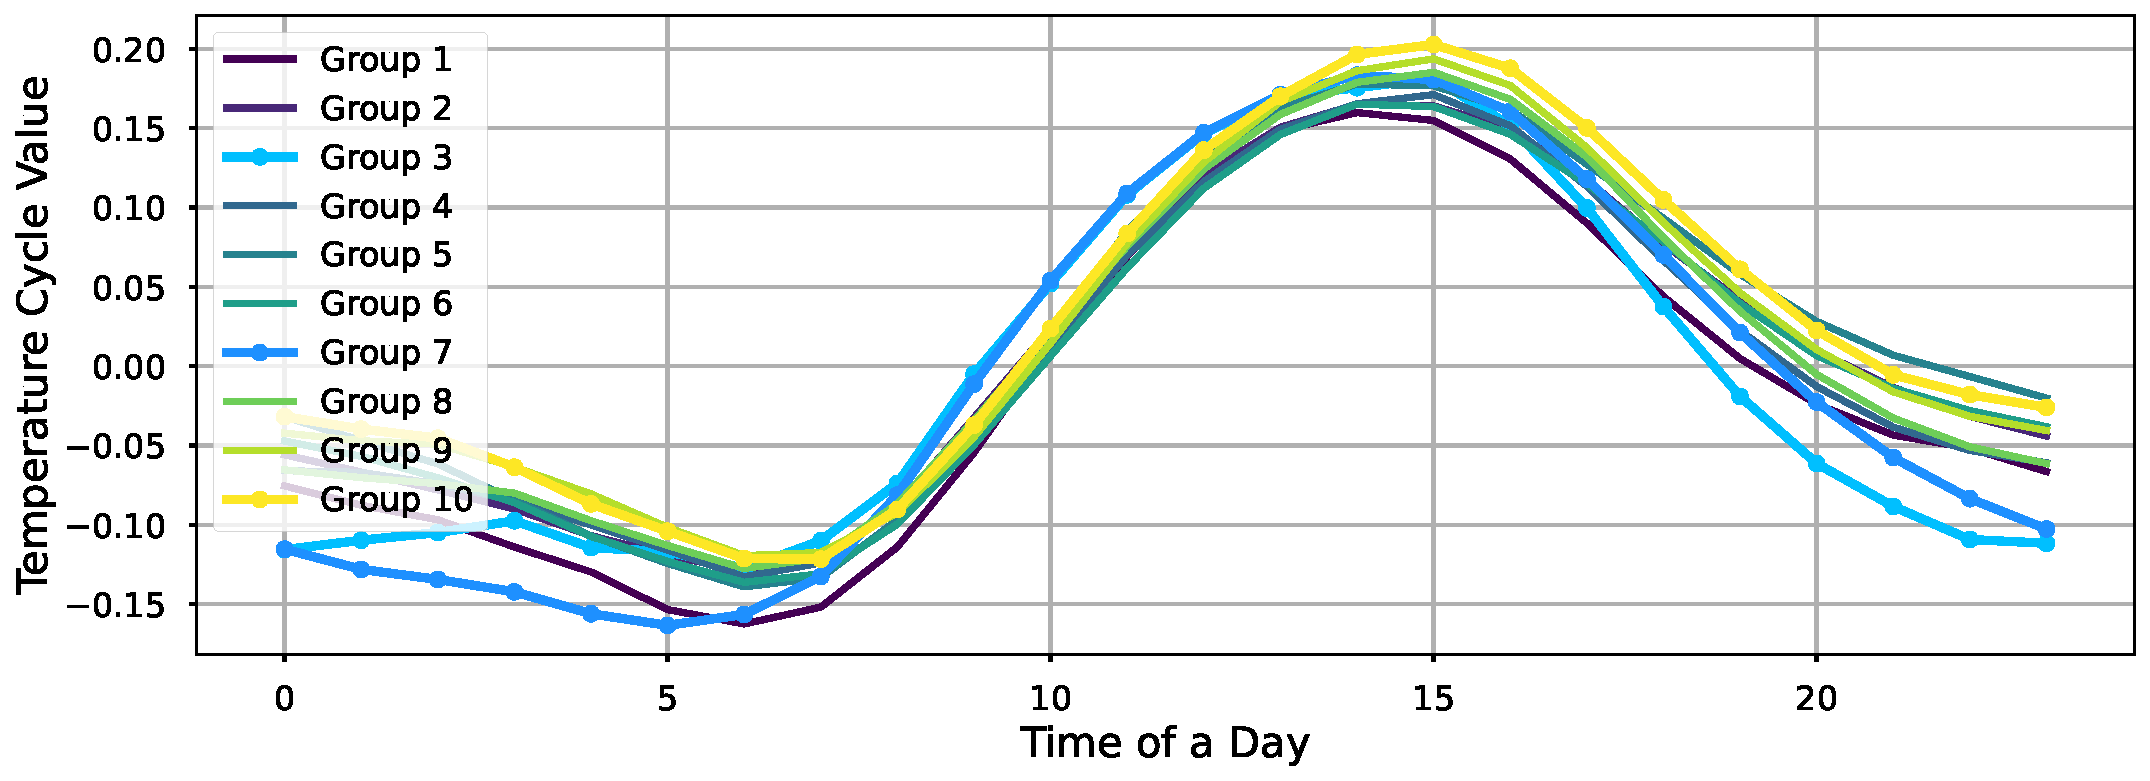
\includegraphics[width=1.0\linewidth]{resources/cycle.pdf}
    \vspace{-2.5em}
    \caption{Daily thermal cycle for different station groups.}
    \label{fig:cycle}
\end{figure}

\textbf{Thermal cycle modeling.} We first visualize the learned daily thermal cycle for different station groups in our cycle learning block. In Figure \ref{fig:cycle}, we observe that the learned daily temperature patterns show that stations warm up before 15:00 PM, cool down at night, and reach their lowest temperatures just before sunrise. This aligns well with the natural temperature patterns typical of Seoul, which has a temperate monsoon climate. Additionally, the differences observed between various station groups accurately reflect the thermal cycle variations in regions with different environments. For example, stations situated in dense urban areas (\underline{Group 10}) consistently show higher regional temperatures, indicating an increased heat risk, while regions with water bodies (\underline{Group 7}) and greenbelt (\underline{Group 3}) display distinctive temperature cycles. These results and observations demonstrate that the thermal cycle learning block, along with our decomposition-based framework, effectively captures clear and precise thermal cycles from noisy historical temperature data.

\begin{figure}[!t]
    \centering
    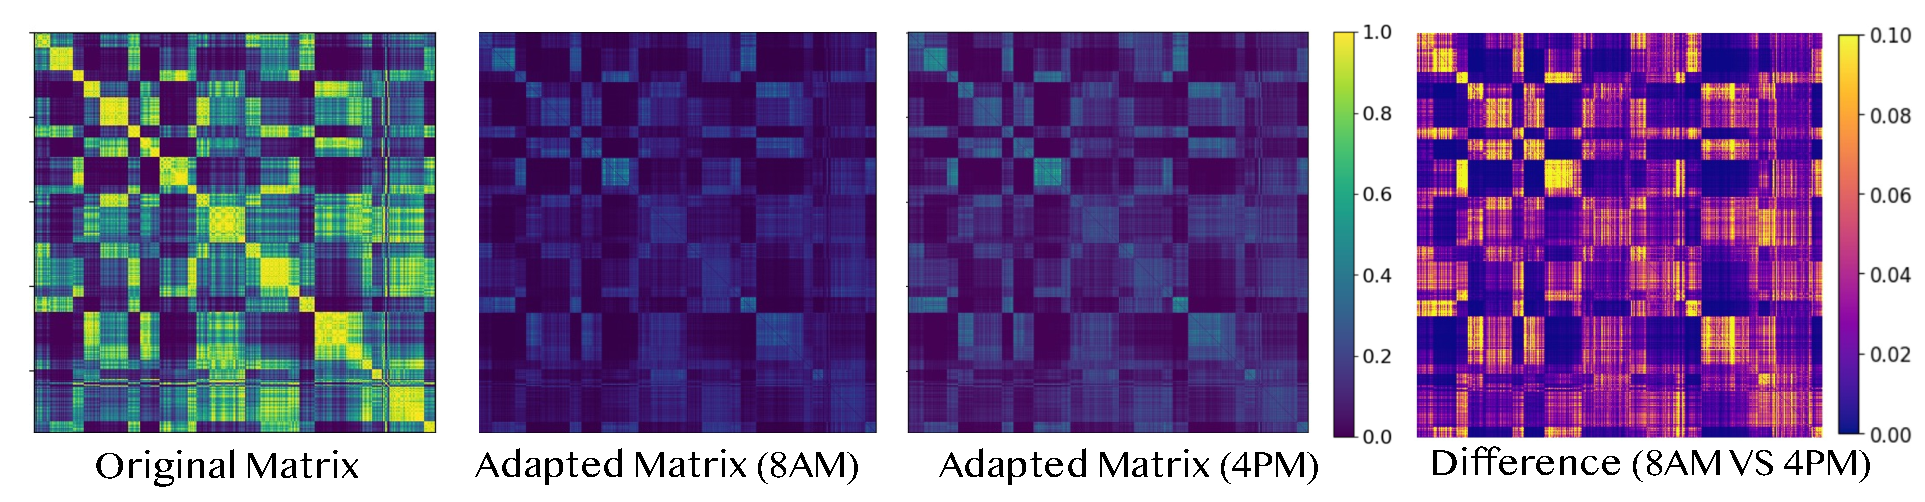
\includegraphics[width=1.0\linewidth]{resources/flow.pdf}
    \vspace{-2em}
    \caption{Adapted adjacent matrix for thermal flow modeling at different time steps.}
    \label{fig:flow}
    \vspace{-1em}
\end{figure}


\textbf{Thermal flow modeling.} In our decomposition-based framework, we utilize spatial graph convolution to model the mechanics of heat flow and introduce a dynamic adaptive adjacency matrix to capture its anisotropy at different time periods. We visualized both the original distance-based adjacency matrix and the learned adaptive matrix for thermal heat flow during the morning, noon, and evening. The differences between the original and learned matrices indicate the anisotropy of spatial heat flow learned by our model, as the vanilla distance-based adjacency matrix is isotropic. Additionally, it is evident that our learned matrix exhibits variations across different time periods, which corresponds well with the dynamic mechanics of thermal flow.

\subsection{Ablation Study (RQ4)}
\begin{figure}[!b]
    \centering
    \vspace{-1em}
    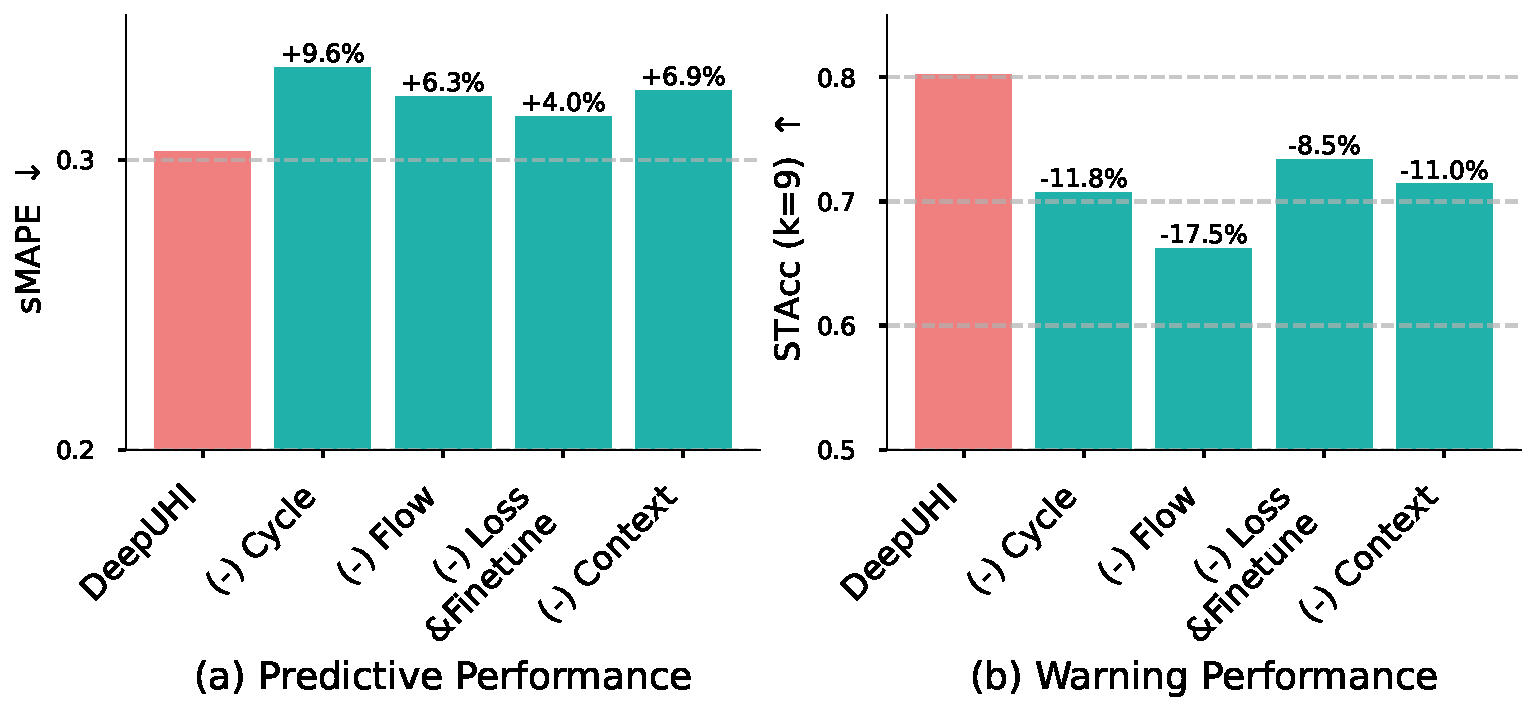
\includegraphics[width=1\linewidth]{resources/ablation.pdf}
    \vspace{-2em}
    \caption{Ablation study on prediction and warning tasks.}
    \label{fig:ablation}
\end{figure}
To investigate the impact of each proposed component of our framework on its performance, we developed the following model variants for an ablation study:
\begin{itemize}[leftmargin=*]
    \item \textbf{(-) Cycle}. This variant removes the thermal cycle learning block and includes no daily cycle decomposing in the framework.
    \item \textbf{(-) Flow}. This variant removes the heat flow learning block and uses a 3-layer MLP for regression.
    \item \textbf{(-) Loss \& Fine-tune}. This variant replaces the variant-aware loss with MSE loss and drops the fine-tuning training strategy.
    \item \textbf{(-) Context}. This variant drops the contextual features for region clustering and regional relations adapting.
\end{itemize}

We report the ablation results of \model and its variants on both temperature prediction and urban heat island (UHI) warning performance in Figure~\ref{fig:ablation}. In summary, our findings are as follows: 1) For the predictive task, thermodynamic modeling plays the most significant role. This indicates that clear daily pattern information can greatly enhance the model's performance in prediction. However, for the warning task, thermal flow modeling is crucial for maintaining high performance. Warning tasks require a deeper understanding of spatio-temporal dynamics, making the dynamic relationship modeling process essential for comprehending complex thermal flows. 2) The variation-aware loss and fine-tuning strategy can improve performance in both tasks to a similar extent. 3) Contextual features can enhance model performance in both tasks; however, if they are excluded, the self-adaptive version of \model still yields satisfactory results.


\vspace{-0.5em}
\section{Real-world deployment}
We deployed the proposed model into the SeoUHI system on the cloud to forecast the Urban Heat Island (UHI) effect. The system comprises four main modules. The data collector module continuously gathers real-time regional temperature data from the SDot project API. To address limited coverage and missing indoor temperature data, the data preprocessing module fills in gaps based on spatio-temporal neighbors. The prediction module forecasts regional temperatures for the next 24 hours at an hourly frequency, while the decision module identifies future hot times and locations, issuing UHI warnings. Additionally, the system automatically sends extreme heat warning emails to registered users during summer to protect vulnerable groups from heat exposure.

\begin{figure}[!b]
\centering
\vspace{-1em}
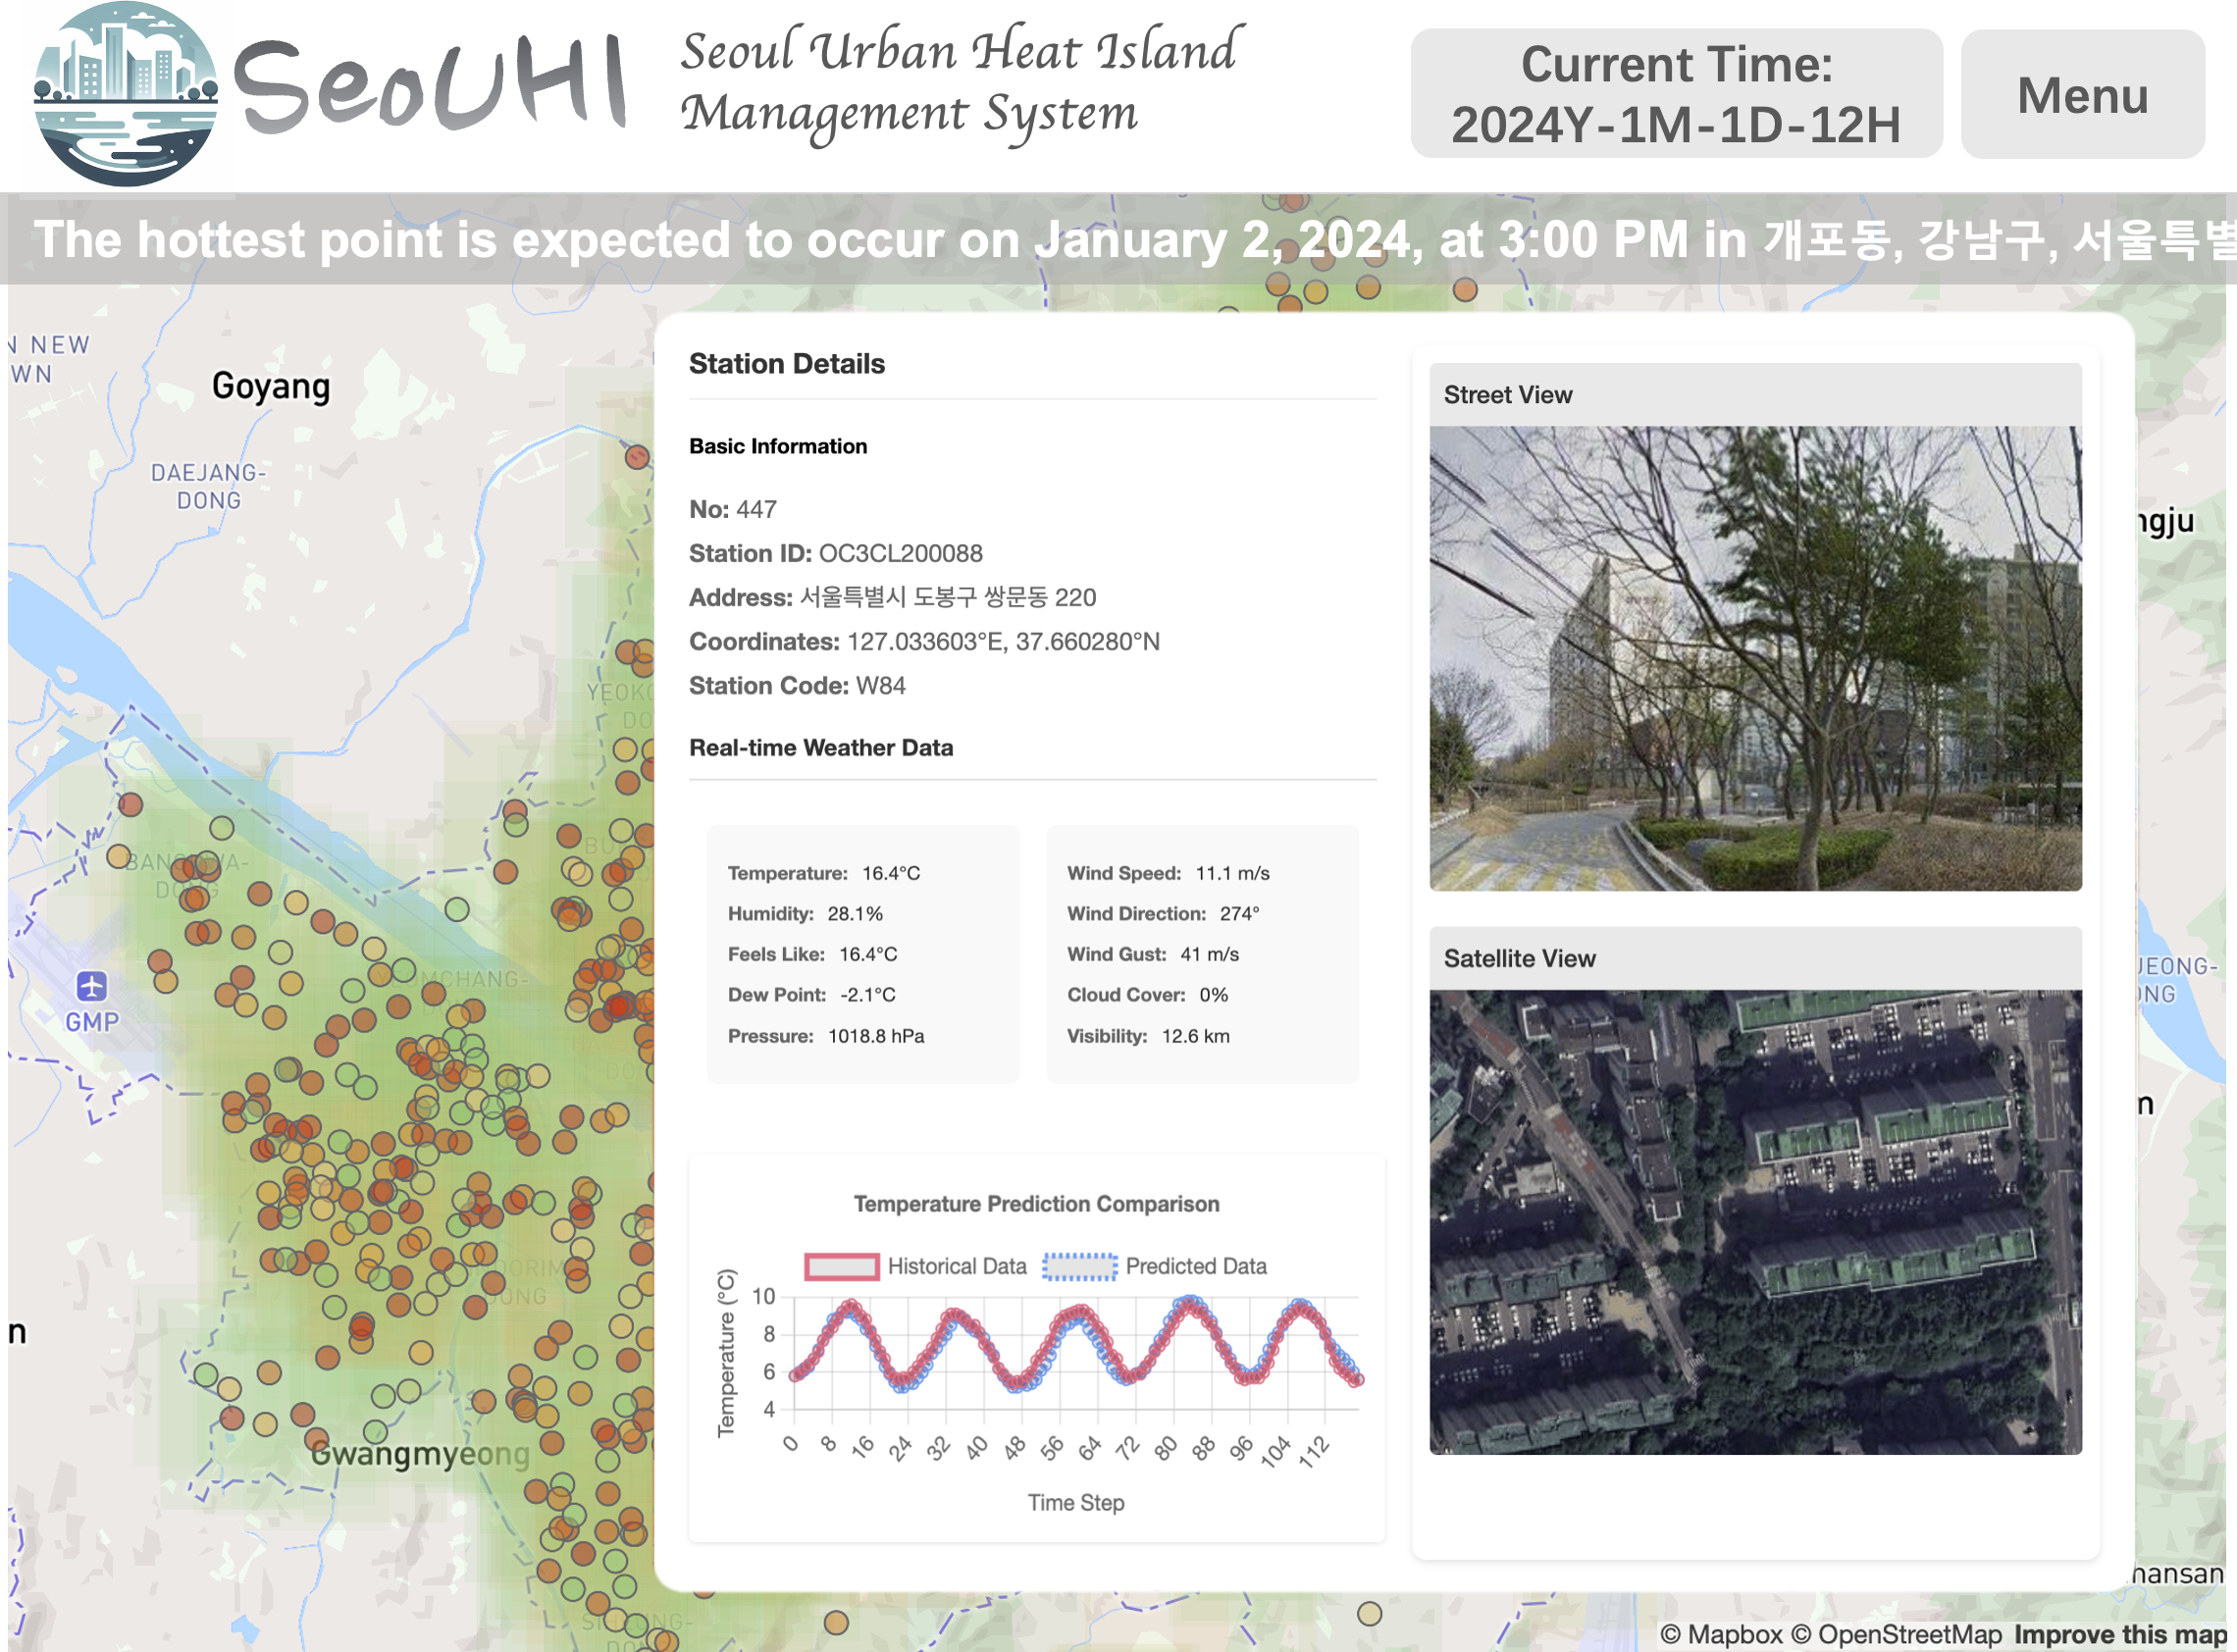
\includegraphics[width=1.0\linewidth]{resources/deploy.png}
\vspace{-2em}
\caption{Web platform of SeoUHI system}
\label{fig:depoly}
\end{figure}

The system features a user-friendly web interface, as shown in Figure \ref{fig:depoly}, displaying a dynamic heat map of Seoul. Users can select a target region to view predicted temperatures in a line graph format, allowing for comparisons between predicted and actual temperatures over different time spans. The predictive system executes hourly updates for the 947 temperature stations in Seoul. To maintain accuracy, the core model is retrained monthly with the latest regional temperature data, benefiting from its lightweight architecture. Our data-driven model does not rely on physical rule-based simulation, eliminating the need for detailed physical information or extensive computational resources, which facilitates practical deployment. However, it requires hourly average regional temperature data, necessitating the installation of temperature sensors within the city, currently limiting deployment to the Seoul area.

\section{Related Works}
\label{sec:relate}
\textbf{Climate Forecasting.} There are two primary approaches for climate forecasting: the physical and statistical approaches. The physical approach, represented by Numerical Weather Prediction (NWP) methods~\cite{bauer2015quiet}, typically requires substantial computational resources to solve simulation equations with boundary conditions. In contrast, statistical approaches, such as GenCast~\cite{price2023gencast}, utilize historical observations to develop large-scale global weather forecasting models that demonstrate superior performance compared to NWP methods. However, both physical and statistical approaches encounter challenges in regional urban climate forecasting, such as UHI effect prediction. At fine-grained scales, physical simulations can become overly complex and time-consuming~\cite{mass1998regional}, while statistical methods are limited to general atmospheric circulation forecasting~\cite{schultz2021can}.


\noindent
\textbf{Multivariate Series Forecasting.} Fine-grain UHI effect forecasting can be approached through multivariate time-series (TS) forecasting or spatio-temporal (ST) forecasting~\cite{shao2024exploring,liu2022contrastive}, the latter of which incorporates spatial information. Deep neural networks, particularly Transformers~\cite{wen2022transformers}, have gained attention in TS forecasting, with models like iTransformer~\cite{liu2023itransformer}, Autoformer~\cite{wu2021autoformer}, and PatchTST~\cite{nie2022time} demonstrating high performance. Fully connected models, such as Dlinear~\cite{zeng2023transformers}, also serve as competitive alternatives.
In spatiotemporal forecasting, STGCN utilizes graph convolution for spatial data processing. STGCN-like models form a broad category of methods capable of addressing both temporal and spatial dependencies~\cite{shao2024exploring,yu2017spatio}, often applied to traffic prediction tasks. Further techniques like STID~\cite{shao2022spatial} offer a simple spatial-temporal identity-attaching approach to capture spatial dependencies without relying on graphs. Recently, there has been a rising trend of building foundation models~\cite{liang2025foundation} for spatio-temporal data science.


\noindent
\textbf{Data-driven Urban Thermal Study.} Contextual environment data like satellite, and street-view imagery are commonly utilized as key data sources to support regional thermal condition studies~\cite{hao2025unlocking,han2024microclimate,hao2025nature}. Existed context data-enhanced techniques often employ regression-based approaches to compute the relation between the local thermal effect and environmental situations. However, the results of these methods are limited to qualitative analysis. \cite{equere2020definition} analysis of the relation between local satellite image and UHI effect and compute the coefficient of determination factor $R^{2}$ of 0.68 between them in San Francisco. \cite{equere2021integration} emphasize the importance of terrain features in UHI spatial inference. \cite{han2024microclimate} incorporate land use data to support the prediction of serval climate situations.
%\vspace{-0.1in}
\section{Conclusion and Future Work}
\label{sec:conclusion}
In this paper, we present DeepUHI, a context-aware thermodynamic modeling framework for fine-grained Urban Heat Island (UHI) effect forecasting. We introduce a data-driven heat decomposition method that captures urban thermodynamics from both thermodynamic cycle and thermal flow perspectives, systematically integrating urban environment data. Empirical results from regional temperature prediction and thermal warning tasks, compared with state-of-the-art baselines, demonstrate the effectiveness of DeepUHI. Additionally, we release the first fine-grained multi-modal field temperature dataset, \textit{SeoulTemp}, and deploy our model on the SeoUHI web platform to support further data-driven studies on micro-climates and solutions for urban sustainability. We hope that this work and dataset inspire future research aimed at generating more data-driven insights and solutions for analyzing or even mitigating the urban heat island effect.



\section*{Acknowledgement}
This work is mainly supported by the Guangdong Basic and Applied Basic Research Foundation (No. 2025A1515011994). This work is also supported by the National Natural Science Foundation of China (No. 62402414), Guangzhou Municipal Science and Technology Project (No. 2023A03J0011), the Guangzhou Industrial Information and Intelligent Key Laboratory Project (No. 2024A03J0628), and a grant from State Key Laboratory of Resources and Environmental Information System, and Guangdong Provincial Key Lab of Integrated Communication, Sensing and Computation for Ubiquitous Internet of Things (No. 2023B1212010007). Additionally, this work benefits from the Red Bird MPhil Program at the Hong Kong University of Science and Technology (Guangzhou).

We would like to extend our special gratitude to PCI Technology Group Co., Ltd. (PCITECH), Guangzhou, China, as well as to Dr. Zheng Chen and Dr. Kai Wang from PCITECH for their valuable support of this work.

\clearpage

\bibliographystyle{ACM-Reference-Format}
\balance
\bibliography{refs}

\appendix 
\section{Appendix}
% \balance
\label{sec:appendix}
\subsection{Components of Variation-aware Loss}
\label{app:loss}
1. \textbf{Amplitude Shifting Invariance}: Implemented using the softmax function to ensure that the gap between the prediction and the ground truth is equal at each step. The formula is as follows:
   \[
   \mathcal{L}_{\text{a.shift}}(Y, \hat{Y}) = \frac{1}{T'} \sum_{i=1}^{T'} \left| 1 - \text{Softmax}(d(y_i, \hat{y}_i)) \right|
   \]
   where \(d(y_i, \hat{y}_i)\) is the signed distance between the true value and the predicted value, and \(T'\) is the length of the sequence.

2. \textbf{Phase Shifting Invariance}: Achieved by utilizing the gap between the Fourier coefficients to retain the dominant frequency components of the original time series while reducing noise in non-dominant frequencies. The formula is as follows:
   \[
   \mathcal{L}_{\text{phase}}(Y, \hat{Y}) = \begin{cases} 
   \left\| F(Y) - F(\hat{Y}) \right\|_p & \text{for dominant freq.} \\
   \left\| F(\hat{Y}) \right\|_p & \text{otherwise}
   \end{cases}
   \]
   where \(F(Y)\) and \(F(\hat{Y})\) are the Fourier transforms of the true and predicted values, respectively, and \(\left\| \cdot \right\|_p\) is the Lp norm.

3. \textbf{Point-wise Distance}: Implemented through the mean average error to measure the average magnitude of the errors in a set of predictions, without considering their direction. The formula is as follows:
   \[
   \mathcal{L}_{\text{distance}}(Y, \hat{Y}) = \frac{1}{T'} \sum_{i=1}^{T'} \left| y_i - \hat{y}_i \right|
   \]
   where \(y_i\) and \(\hat{y}_i\) are the true and predicted values at time step \(i\), respectively, and \(T'\) is the length of the sequence.



\subsection{Spatio-temporal Periodicity.}
In this work, we develop a thermodynamic model of the urban heat island effect primarily using a historical spatio-temporal field temperature dataset. To manage the complex variations in thermal issues, we integrate thermal equations to guide our model and simplify the modeling process through an equation-based decomposition framework. We introduce the design of each component from a thermal modeling perspective and demonstrate their effectiveness in the paper. 

\begin{figure*}[!t]
    \centering
    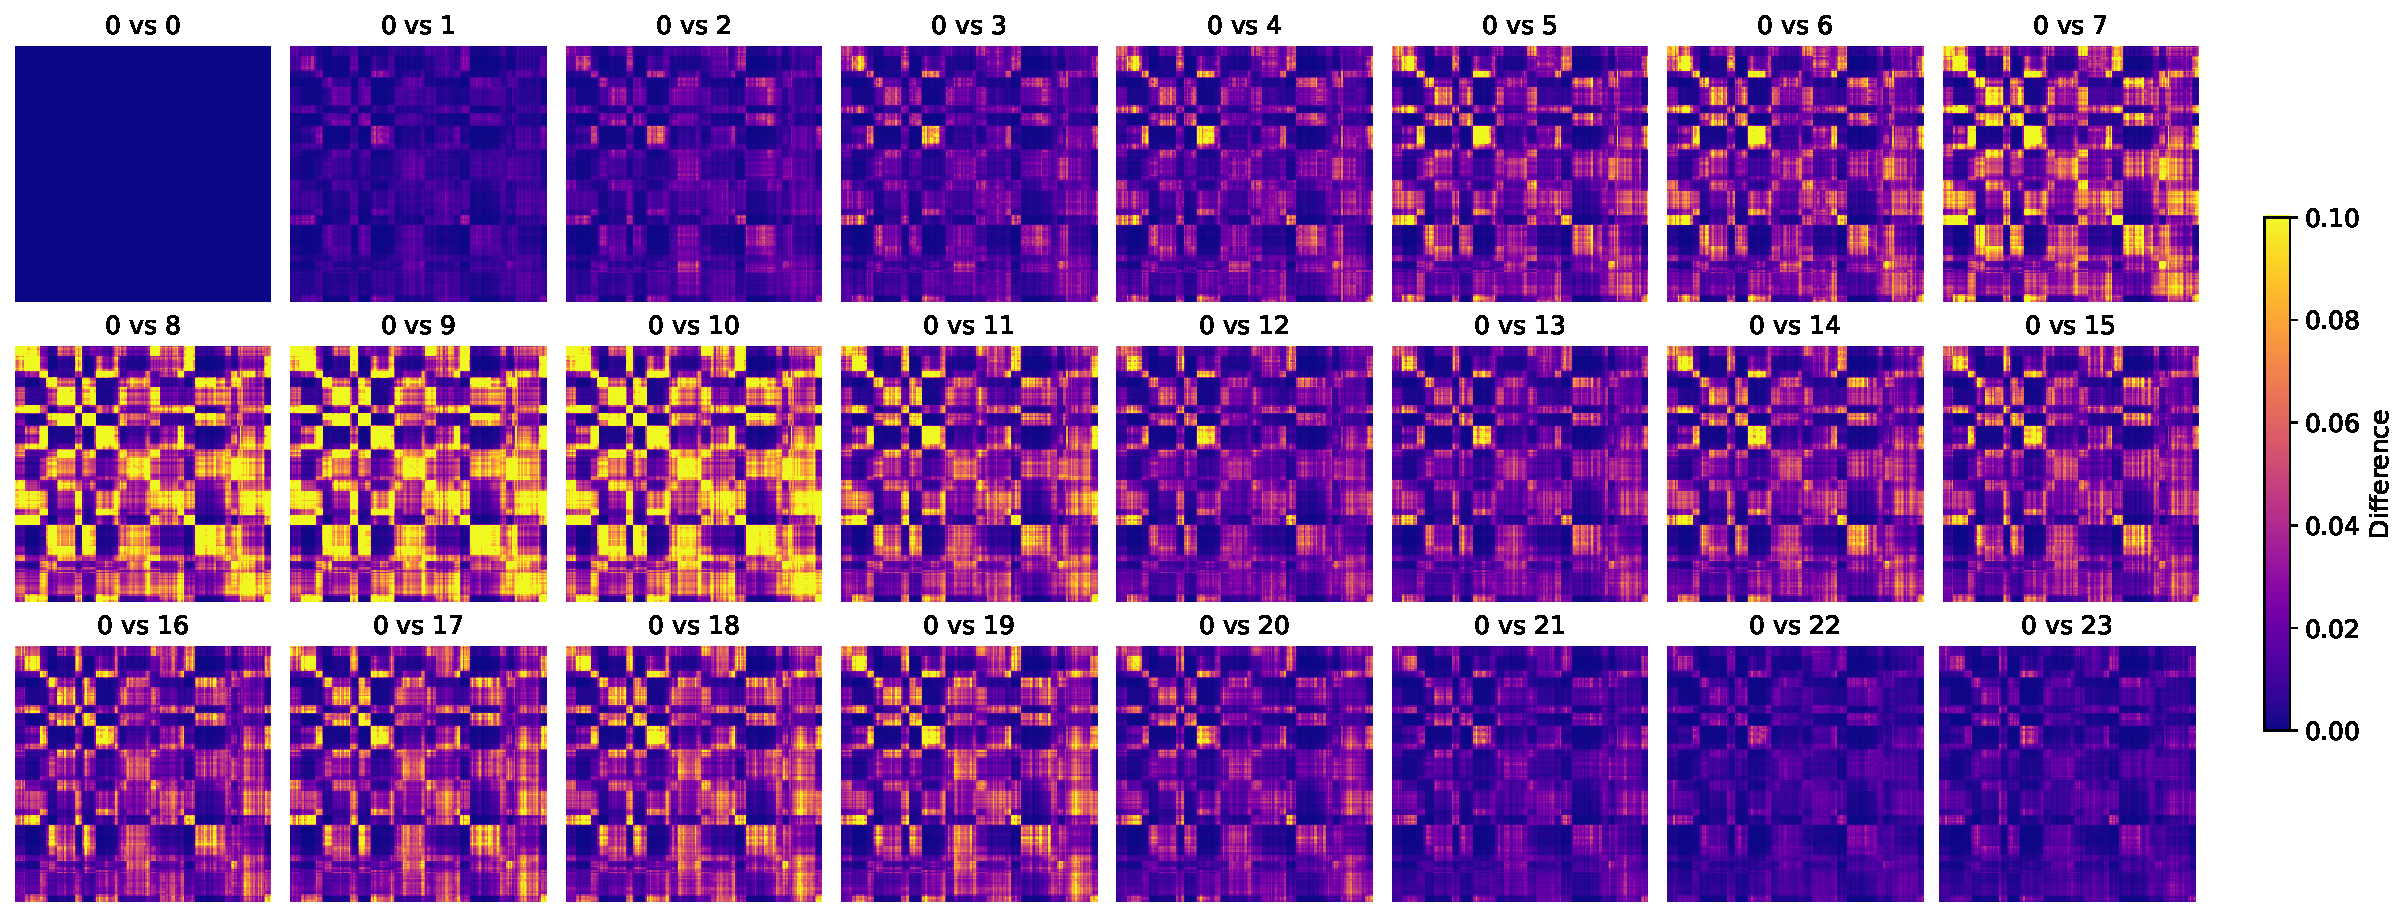
\includegraphics[width=0.95\linewidth]{resources/flow_cycle.pdf}
    \vspace{-1em}
    \caption{Spatio-relation Periodicity: daily variation of the learned adjacency matrix}
    \label{fig:flow_cycle}
\end{figure*}

However, from a data-driven spatio-temporal forecasting perspective, some parameter designs based on thermal principles may still require further experimental validation. Specifically, our model is designed to leverage the spatio-temporal periodicity of field temperature data. Below, we will present additional experimental evidence regarding the spatio-temporal periodicity of temperature data.


\begin{figure}[!h]
    \centering
    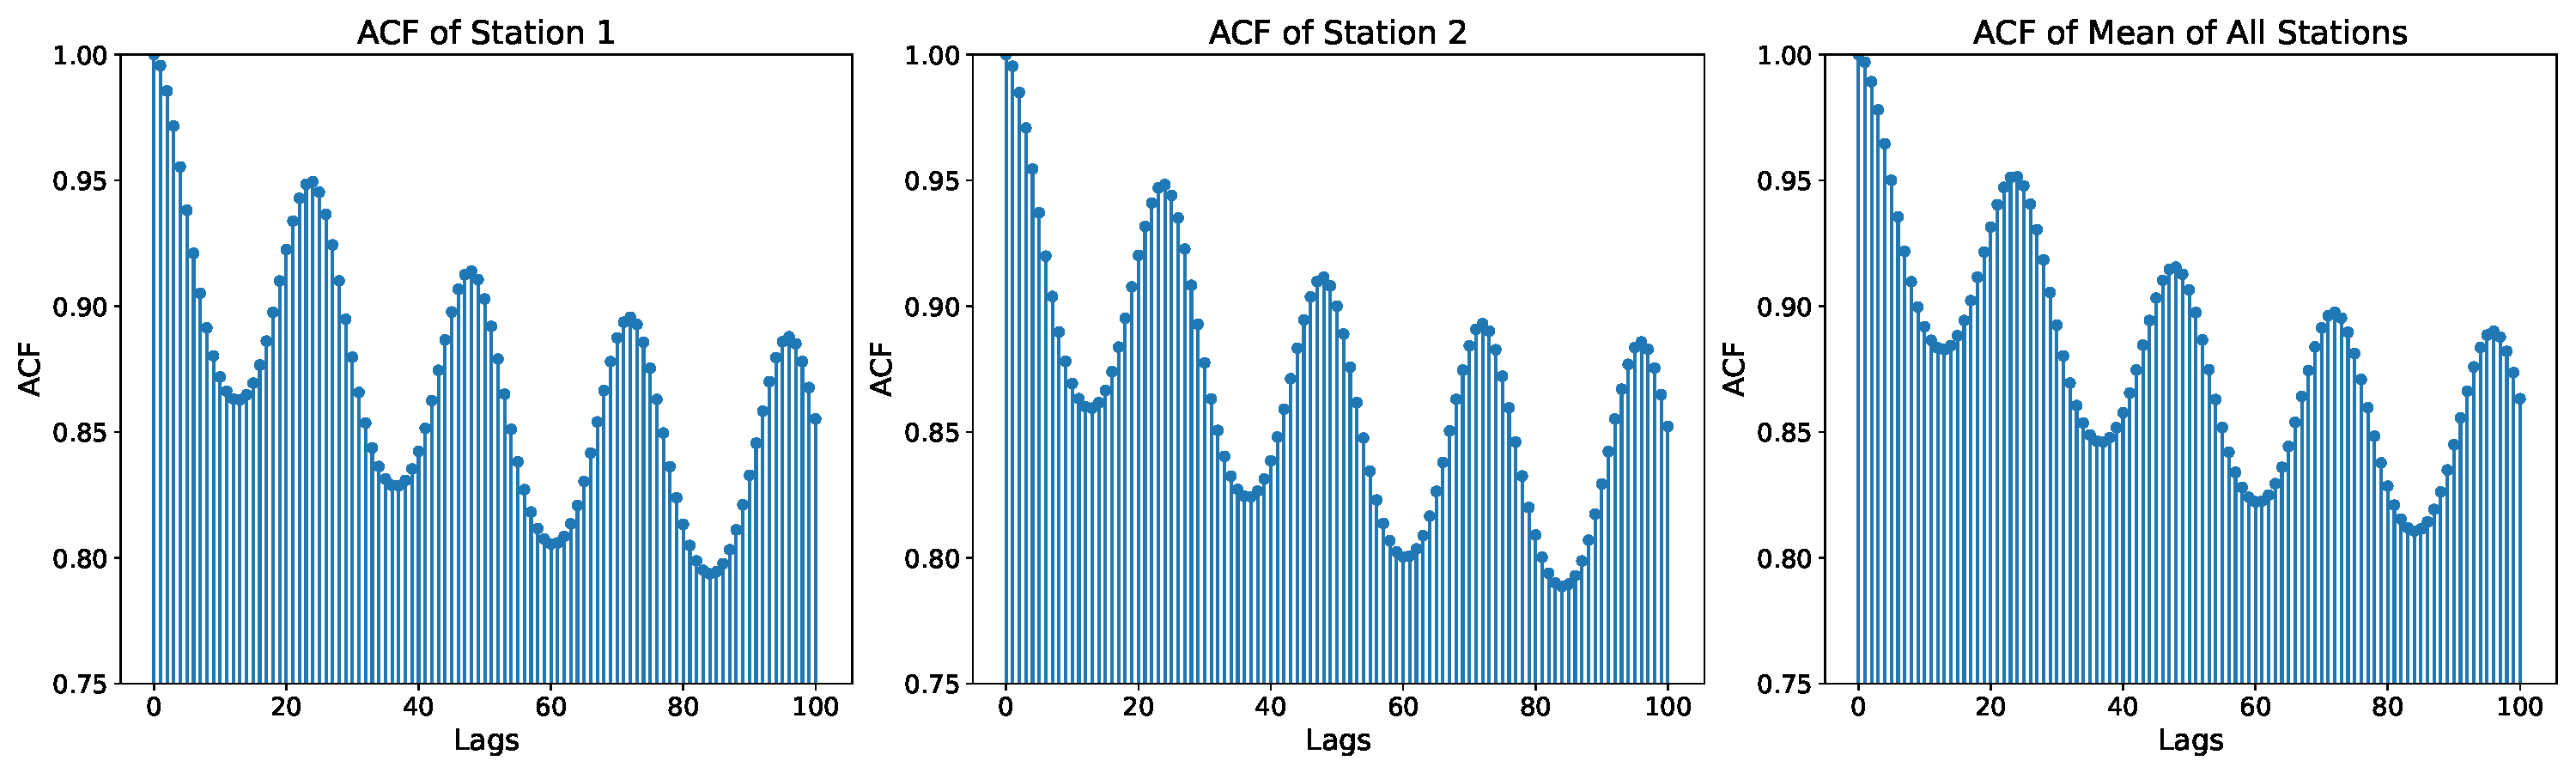
\includegraphics[width=0.95\linewidth]{resources/ACF.pdf}
    \caption{Intra-region Temporal Periodicity: visualization of ACF results on \textit{SeoulTemp} Dataset}
    \label{fig:acf}
\end{figure}

\textbf{Spatio-relation Periodicity.} In Section \ref{sec:spatial_cycle}, we efficiently model the temporal periodic dynamics of \textbf{thermal flow} by setting a period \underline{$W=24$ (daily)}. This approach simplifies the modeling of the temporal dynamics of inter-region spatial correlation, allowing us to focus on daily variations rather than the entire time period, given the daily periodicity of thermal flow dynamics. To validate this periodicity within the data, we present the daily variation of the learned adjacency matrix in DeepUHI over the course of a day in Figure \ref{fig:flow_cycle}. The visualization results further demonstrate the necessity of modeling the temporal dynamics of spatial relations in thermal flow. Notably, the daily variation exhibits a self-regressive trend; the difference between matrix at time period 0 and other periods vary during warning and cooling time within a day but return to the initial state by the end of the day. This observed spatio-relation periodicity in the data-driven training reinforces the rationale behind our design.




\textbf{Intra-region Temporal Periodicity} In Section \ref{sec:temporal_cycle}, we model the intra-region thermodynamics by proposing learnable daily cycles with a cycle length of \underline{W=24} for $\mathbf{Q}$. This approach allows us to concisely model the basic thermodynamic variations. We utilize the autocorrelation function (ACF)~\cite{madsen2007time} to provide statistical support for our model design from a data perspective.

The autocorrelation function (ACF) is a powerful mathematical tool that helps detect periodicity within the data. It measures the correlation between a time series and its lagged values, indicating the presence of autocorrelation within the dataset. Mathematically, this can be expressed as:

\begin{equation}
ACF = \frac{\sum_{t=1}^{N-k}(x_t - \bar{x})(x_{t+k} - \bar{x})}{\sum_{t=1}^{N}(x_t - \bar{x})^2},
\end{equation}

where \( N \) represents the total number of observations, \( x_t \) denotes the value of the time series at time \( t \), \( k \) is the lag time, and \( \bar{x} \) is the mean of the time series values.

When the lag time \( k \) aligns with the cycle of the data, the ACF value exhibits a significant peak. Specifically, the largest peak corresponds to the lag that matches the length of the maximum cycle present in the dataset. Conversely, if the data lacks periodicity, no significant peaks or troughs will be observed.


We present the ACF results for the SeoulTemp dataset in Figure \ref{fig:acf}. It can be observed that intra-region temperature variations display evident periodicity, indicated by prominent peaks and troughs in the plots. More importantly, the maximum cycles shown in the plots align with our pre-inferred cycle length of \underline{W=24}. This finding further supports the validity of our parameter design.


\end{document}
